%!TEX TS-program = xelatex
%!TEX encoding = UTF-8 Unicode

\documentclass[
	12pt,
	twoside,
	openright
	]{book}

\usepackage[
	top=1in,
	bottom=1in,
	inner=1in,
	%margin=1.23in,
	textwidth=13cm,
	%right=7cm
	%showframe
	]{geometry}

\geometry{a4paper}

\usepackage[parfill]{parskip}
\usepackage{graphicx}
\usepackage{epstopdf}
\epstopdfsetup{update}
\usepackage[usenames]{color}
\usepackage{amssymb}

\usepackage{titlesec}
\usepackage{titling}

\newcommand{\hsp}{\hspace{19pt}}
\titleformat{\chapter}[hang]{\Huge\bfseries\sffamily}{\thechapter\hsp•\hsp}{0pt}{\Huge\bfseries\sffamily}

\usepackage{listings}

\usepackage{
	fontspec,
	xltxtra,
	xunicode
	}

\usepackage{
	xfrac,
	unicode-math
	}

\defaultfontfeatures{Mapping=tex-text}
\setromanfont[
	Mapping=tex-text
	]{Rubik Light}
\setsansfont[
	Scale=MatchLowercase,
	Mapping=tex-text
	]{Open Sans}
\setmonofont[
	Scale=MatchLowercase
	]{Andale Mono}
\setmathfont[
	Scale=MatchLowercase
	]{Libertinus Math}

\newfontfamily\quotefont[
		Scale=MatchLowercase,
		Mapping=tex-text,
		LetterSpace=5.0,
		%Scale=1.123,
		]{Open Sans Light}%{Fira Sans Light}

\usepackage{etoolbox}
\AtBeginEnvironment{quote}{\quotefont\small}

\usepackage[
	autostyle,
	italian=guillemets,
	% altre opzioni
	]{csquotes}

\usepackage[
	english,
	italian
	]{babel}

\usepackage{imakeidx}
\makeindex
%\makeindex[name=things, title=Indice analitico]

\usepackage{tabularx}
\usepackage{array}
\newcolumntype{L}[1]{>{\raggedright\let\newline\\\arraybackslash\hspace{0pt}}m{#1}}
\newcolumntype{C}[1]{>{\centering\let\newline\\\arraybackslash\hspace{0pt}}m{#1}}
\newcolumntype{R}[1]{>{\raggedleft\let\newline\\\arraybackslash\hspace{0pt}}m{#1}}

\usepackage{longtable}
\usepackage{multirow}
\usepackage{booktabs}

\usepackage{paralist}

\usepackage{tikz}
\usetikzlibrary{
  angles,
  quotes,
  decorations.pathmorphing,
  decorations.markings}
\usepackage{pgfplots}

\usepackage{wrapfig}

\usepackage{url}

\linespread{1.1}

\renewcommand{\arraystretch}{1.6}

\newfontfamily\csdb[Ligatures=TeX]{Alegreya}

\usepackage{changepage}

\usepackage{ragged2e}

\usepackage[
	style=authoryear,
	%backend=biber
]{biblatex}

\addbibresource{musebib/nono-luigi.bib}
\addbibresource{musebib/novecento.bib}
%\addbibresource{musebib/partiture/milestone.bib}

% ----------------------------------------------------–––––––––– LISTING

% Make LaTeX output a dot when typing an asterisk
%\DeclareMathSymbol{*}{\mathbin}{symbols}{"01}

% lstlistings setup
\definecolor{yobg}{rgb}{0.9,0.9,1}
\definecolor{yotxt}{rgb}{0.01,0.01,0.52} % a dark blue.
\definecolor{mylstbg}{rgb}{0.98,0.98,0.98} % a really pale grey.
\definecolor{mylstcmt}{rgb}{0.01,0.52,0.01} % a dark green.
\definecolor{mylstdoc}{rgb}{0.80,0.30,0.80} % a medium pink.

\lstset{%
  language=C++,
  numbers=left,%none,
  tabsize=4,
  %frame=single,
  breaklines=true,
  numberstyle=\tiny\ttfamily,
  backgroundcolor=\color{mylstbg},
  basicstyle=\footnotesize\ttfamily,
  commentstyle=\slshape\color{mylstcmt}, %\itshape,
  %frameround=tttt,
  columns=flexible, %fixed,
  showstringspaces=false,
  emptylines=2,
  inputencoding=utf8,
  extendedchars=true,
  literate=	{á}{{\'a}}1
			{à}{{\`a}}1
			{ä}{{\"a}}1
			{â}{{\^a}}1
			{é}{{\'e}}1
			{è}{{\`e}}1
			{ë}{{\"e}}1
			{ê}{{\^e}}1
			{ï}{{\"i}}1
			{î}{{\^i}}1
			{ö}{{\"o}}1
			{ô}{{\^o}}1
			{è}{{\`e}}1
			{ù}{{\`u}}1
			{û}{{\^u}}1
			{ç}{{\c{c}}}1
			{Ç}{{\c{C}}}1,
  emph={component, declare, environment, import, library, process},
  emph={[2]ffunction, fconstant, fvariable},
  emph={[3]button, checkbox, vslider, hslider, nentry, vgroup, hgroup, tgroup, vbargraph, hbargraph, attach},
  emphstyle=\color{yotxt}, %\underline, %\bfseries,
  morecomment=[s][\color{mylstdoc}]{<mdoc>}{</mdoc>},
  rulecolor=\color{black}
}

% ----------------------------------------------------–––––––––– CUSTOM COMMANND
\newcommand*\rfrac[2]{{}^{#1}\!/_{#2}}

\newcommand{\rb}{\index{Rumore Bianco}\emph{rumore bianco}}
\newcommand{\tz}{\index{Trasformata zeta}\emph{trasformata zeta}}

% ----------------------------------------------------
% ----------------------------------------------------
% ----------------------------------------------------

\begin{document}

%%!TEX TS-program = xelatex
%!TEX encoding = UTF-8 Unicode
%!TEX root = ../../../LSSN.tex

%------------------------- COMANDO TIKZ
\newcommand\Base[1][0]{
\begin{scope}[xshift=#1]
\clip
  (-0.5,5.5) rectangle (5.5,-0.5);
  \draw[->]
  (-0.5,0) -- (5,0) node[right] {$u$};
\draw[->]
  (0,-0.5) -- (0,5) node[above] {$v$};
\coordinate (O) at (0,0);
\coordinate (aux1) at (40:4);
\coordinate (aux2) at (aux1|-0,0);
\coordinate (aux3) at (4,{4*tan(40)});
\draw
  (O) -- (aux3) -- (aux3|-0,0)
  (aux1) -- (aux2);
\draw[
	thick,
	%red!70!black
	]
  (O) circle (4);
\pic[
	draw,
	"$x$",
	angle radius=30pt,
	angle eccentricity=1.2
	]{angle = aux2--O--aux1};
\end{scope}
}
%------------------------- COMANDO TIKZ


%!TEX TS-program = xelatex
%!TEX encoding = UTF-8 Unicode
% !TEX root = ../METM.tex

%------------------------- COPERTINA
\begin{center}
	\fontsize{40}{40}{\csdb MUSICA} \\
	\fontsize{40}{40}{\csdb ELETTRONICA} \\
	\fontsize{40}{40}{\csdb TECNOLOGIA} \\
	\fontsize{40}{40}{\csdb MUSICALE}\\[-.31cm]
	\noindent\makebox[\linewidth]{\rule{.51\paperwidth}{1pt}}
	%\fontsize{19}{19}\selectfont{Pasquale CITERA} 	\\
	%\fontsize{19}{19}\selectfont{Marco Matteo MARKIDIS} 	\\
	\fontsize{19}{19}\selectfont{Giuseppe SILVI} 	\\
	\vfill
	\fontsize{13}{13}\selectfont{APPUNTI} \\
	%\fontsize{13}{13}\selectfont{Liceo Musicale S. SATTA di NUORO} \\
	\fontsize{13}{13}\selectfont{\emph{draft - \today}} \\
\end{center}
\thispagestyle{empty}
\clearpage
~ \vfill
blank page
\thispagestyle{empty}
\clearpage
%------------------------- COPERTINA


\clearpage

\tableofcontents

\raggedright

%!TEX TS-program = xelatex
%!TEX encoding = UTF-8 Unicode
% !TEX root = ../metp.tex

\chapter*{MANIFESTO}
\addcontentsline{toc}{chapter}{MANIFESTO}

%\begin{adjustwidth}{23mm}{0mm}

Questo lavoro deriva dall'esigenza di organizzare un testo che possa
ristabilire un equilibrio scolastico e, con un po' di presunzione, artistico,
nelle attività didattiche inerenti la Musica Elettronica e le Tecnologie
Musicali. Non è propriamente un manuale quanto una raccolta organizzata di
appunti che seguano un percorso chiaro e progressivo attraverso gli anni di
studio della materia.

L'esigenza di mettere in un contenitore questi materiali viene direttamente
dal percorso d'insegnamento in diversi gradi del percorso formativo elettroacustico.
La bibliografia specifica è ricca ed in continua evoluzione data la materia
viva che la alimenta. Nonostante questo, in lingua italiana, i testi attualmente di
riferimento hanno un assetto ludico, d'intrattenimento. Organizzati ad
unità come fossero un corso di lingua, a livelli, trasformano argomenti musicali
in attitudini ricreative, rafforzando l'idea di didattica applicata alla base
di troppe classi di musica elettronica in Italia.

Un riferimento letterario, ad indirizzo opposto, è il testo di Walter Branchi
\emph{Tecnologia della Musica Elettronica} che dal lontano 1975 ancora riesce
a suggerire un'idea di didattica organica e progressiva ineguagliata, con i
difetti di un'opera prima in tutti i sensi, ma con la prospettiva dello studio
scolastico organizzato. A questo testo si ispira questa raccolta, \emph{METP},
all'idea di un percorso di comprensione che viene da un'idea di scuola,
senza la pretesa di creare un abile manovratore di pomelli in ogni possibile lettore.
Le problematiche essenziali sono altre e sono, sempre prendendo spunto dal lavoro di Branchi,
ancora egregiamente espresse dalle parole di Domenico Guaccero nella prefazione:

\begin{quote}
  \ldots val la pena ricordare e mantenere fermi gli apporti che la “musica
  elettronica” ha introdotto nell'opera musicale\ldots E cioè l'andare alla
  radice del suono, come fatto fisico e (ache) da qui come fatto musicale, la
  possibilità di liberarsi definitivamente dal “dover costruire” sitemi
  intervallari, il porre il problema del rapporto musica esecutore e musica
  spettacolo in termini fino allora inusitati, di riproporre, ma allargandone
  permamentemente i confini, il rapporto tra tecnologia e composizione.
\end{quote}

In questa ottica di indagine, alla \emph{radice del suono}, ci si pone
trasversalmente, lungo il periodo d'apprendimento di uno studente, a qualsiasi
livello. Non è dunque la quantità di nozioni (o unità) che si collezionano con
la lettura, quanto la qualità dell'esperienza formativa a tracciare il percorso.

\begin{quote}
  Cominciare con uno studio del “tempo” e delle "onde"\ldots È li che comincia
  il moto, quindi il suono. È li che musicista e tecnico cominciano ad
  incontrarsi. Prima di tutte le cognizioni di acustica ed elettroacustica o di
  tecnologia elettronica, è li che si può misurare quello che diventa il "nuovo"
  tecnico-musicale itrodotto tramite i mezzi elettronici: com'è stato detto, si
  tratta di "comporre il suono, non comporre col suono".
\end{quote}

La composizione come materia di studio sembra non appartenere più alle classi di
tecnologia. Il mezzo tecnico ha completamente inebriato le menti e distolto
l'attenzione dall'\emph{osservazione mediante composizione} di ciò che percepiamo,
ovvero, ancora: il suono. Uno studente agli inizi del proprio percorso potrebbe
affrontare un esercizio compositivo se gli si fornissero le regole di
comprensione del proprio operato e della relazione di questo con il mondo percepito, per

\begin{quote}
  \ldots andare alla radice del suono. In quest'ambito possono avere più senso
  i vari problemi, come quello di mirare a costruire timbri nuovi\ldots studiare
  per analisi, gli strumenti naturali, in maniera da usare gli strumenti naturali
  come termini di confronto cui l'orecchio è abituato, cioè scritti in codice
  forte.

  Dalla radice del suono, come fatto fisico, si può passare alla radice della
  percezione e della realizzazione sonora.
\end{quote}

Negli anni di scuola superiore, del Liceo, questa metodologia è adottata
\emph{naturalmente}. Sarebbe troppo semplice parlare di materie scientifiche
quali la fisica, la biologia, la chimica per creare paralleli tra percepito,
analizzato e compreso. Girandoci più alla larga possibile potremmo parlare di
latino e italiano, di letteratura. Di imparare a scrivere attraverso la storia
della scrittura, dei meccanismi che hanno resistito alla storia per finire nel
linguaggio comune. Nella musica elettronica, nelle tecnologie musicali, nei
libri ad unità, si procede per atemporalità, per meccanismi e tecnicismi avulsi
dall'essere nel tempo delle cose. Si spiegano le tecniche senza su queste fare
quello che si fa in italiano, scrivere, comporre temi. Come se la composizione
fosse una questione esclusiva dei compositori.

Insegnare a comporre, a scrivere, attraverso il ragionameto, è un esattamente
una questione tecnica

\begin{quote}
  faranno bene ad essere quanto più rigorosi teoriocamente e quanto più
  preparati tecnologicamente, in maniera da poter maneggiare tutte le
  apparecchiature possibili\ldots È la via della didattica, quella a cui
  intelligentemente si rifà questo libro di Branchi\ldots

  Esso non è un testo pensato a priori per insegnare le tecniche elettroniche,
  ma è \emph{il risultato} d'una attività didattica già effettuata\ldots Non
  un'aggiunta all'erudizione o un contributo all'indagine teorica, ma, più
  semplicemente e pertinemtemente, uno strumento di lavoro, da utilizzare nella
  pratica.
\end{quote}

Questo lavoro ha la presunzione di non servire a niente se lo scolpo della
lettura è un'apprendimento collezionistico di espedienti e meccanismi.

Questo lavoro vuole e può fornire meccanismi mentali di indagine,
sperimentazione, speculazione, comprensione e composizione che \emph{una scuola}
dovrebbe innestare in alcuni studenti, in alcuni individui. Non in tutti, come nei
corsi di lingua di base, una unità alla volta, ma solo quelli che da questi
ragionamenti possano alzare gli occhi per scoprire di aver
cambiato il proprio modo di percepire le relazioni tra le cose.

***

Questo testo, pur prendendo prezioso esempio dalle pagine di Branchi, vuole fare
diversi passi in molteplici altre direzioni. La distanza temporale dal testo di
Branchi ci permette di guardare a nuovi modi di fare didattica. Il più
importante ed efficae è quello del libero accesso al codice, alla libera
partecipazione al progetto per un'informazione aperta alla discussione.

Questo testo è quindi open source, il progetto risiede all'indirizzo
\url{https://github.grammaton.io/metp}. Atteaverso questo indirizzo si può
partecipare alla scrittura, all'integrazione, alla discussione al fine di
rendere il testo vivo, in continua composizione.

Please note that this project is released with a Contributor Code of Conduct.
By participating in this project you agree to abide by its terms.

%\end{adjustwidth}

\clearpage


\input{CAPITOLI/0001-COC}

%!TEX TS-program = xelatex
%!TEX encoding = UTF-8 Unicode
% !TEX root = ../../metp.tex

\chapter{FENOMENI}
\startcontents[chapters]
\printcontents[chapters]{}{1}{}

~\vfill

\begin{flushright}
		\textit{Nihil est in intellectu quod prius non fuerit in sensu}\footnote{
		Locuz. lat. \emph{niente è nell’intelletto, che prima non sia stato nei sensi},
		usata come assioma nella filosofia scolastica. Accolta da Locke nella
		sua teoria sull’origine delle idee, fu integrata da Leibniz con
		l’aggiunta \emph{nisi ipse intellectus} \emph{(eccetto l’intelletto stesso)}. --
		\url{treccani.it}}
	\end{flushright}

\bigskip

Il \emph{primo passo} che l'uomo compie, ciclicamente, verso la comprensione del
mondo sonoro che lo circonda è cambiato innumerevoli volte durante la storia degli
ultimi 3000 anni ed è sempre stato un passo mosso di pari passo con la musica,
la sua storia, la sua funzione culturale.

In Europa, solo nel novecento, possiamo segnalare differenti approcci alla
comprensione del mondo sonoro prima e dopo le guerre, prima e dopo la radio-televisione,
prima e dopo il calcolatore digitale, prima e dopo l'automobile come bene primario.

%Varese:
%Turing:

Oggi si può ascoltare e cominciare a parlare di suono cercando di unire discipline diverse
che trattano il tema scientificamente, tra cui, la musica, ormai è una di queste.
Il primo oggetto analizzabile da questo punto di vista è proprio l'oscillazione nel tempo,
il moto che da vita alla materia in vibrazione.

\clearpage

%!TEX TS-program = xelatex
%!TEX encoding = UTF-8 Unicode
%!TEX root = ../../metm.tex

\section{Oscillazioni}

Osservando, anche ad occhi chiusi, una ruota panoramica potremmo dire che
completa una rotazione ogni 30 minuti. Osservando ancora il comportamento di
questa ruota panoramica notiamo che questa compie un giro ogni 30 minuti,
ovvero completa un ciclo di rotazione tornando al punto di partenza e poi
ripete questa rivoluzione più volte. Questo è un esempio di funzione periodica,
perché la ruota panoramica ripete la sua rivoluzione, o ciclo, ogni 30 minuti
e quindi diciamo che ha un periodo di 30 minuti.

\input{CAPITOLI/0100/TIKZ/0101-pan}

Osservate ancora la ruota panoramica, si muove in senso antiorario. C'è una
sola cabina occupata, seguiamola. Volendo prendere nota dell'altezza di quella
cabina durante i trenta minuti che impiega a tornare al punto di partenza,
seguendola disegneremmo una linea, probabilmente verticale, che va dall'altezza
minima all'altezza massima.

%!TEX TS-program = xelatex
%!TEX encoding = UTF-8 Unicode

%------------------------- IMMAGINE TIKZ
\begin{tikzpicture}[scale=.99]
  \draw[->] (0,-2.5) -- (0,2.5);
  \draw[->] (-2.5,0) -- (2.5,0);

\draw[
  postaction={
    decorate,decoration={
      markings,
      mark=at position 0.19 with {\arrow[line width=1mm]{>}},
      mark=at position 0.69 with {\arrow[line width=1mm]{>}}}},
    thick
] (0,0) circle (2);

\coordinate (A) at (2,0);

\filldraw (A) circle (2pt) node[above right] {00'};
\filldraw (A) circle (2pt) node[below right] {30'};

\coordinate (B) at (90 : 2);

\filldraw (B) circle (2pt) node[above left] {Cabina};

\draw (4,-2) -- (4,2);

\coordinate (C) at (4,0);
\coordinate (D) at (4,2);
\coordinate (F) at (4,-2);

\filldraw (C) circle (2pt) node[above right] {0};
\filldraw (D) circle (2pt) node[above right] {altezza massima};
\filldraw (F) circle (2pt) node[below right] {altezza minima};

\coordinate (E) at (270 : 2);

\filldraw (E) circle (2pt) node[below right] {Cabina};

\draw[dashed] (0,2) -- (4,2);
\draw[dashed] (0,-2) -- (4,-2);
\end{tikzpicture}
%------------------------- IMMAGINE TIKZ


Se decidessimo che il nostro foglio avesse non una, come nella descrizione
precedente, ma due dimensioni di rappresentazione, l'altezza ed il tempo, e
quindi seguissimo con lo sguardo la cabina ed annotando l'altezza spostassimo
simultaneamente ed a velocità costante il foglio, simulando lo scorrimento del
tempo, il disegno finale dovrebbe apparire come un'onda.

\input{CAPITOLI/0100/TIKZ/0103-pan}

Con la rappresentazione dell'onda descriviamo un'oscillazione, ovvero un moto
periodico attorno alla posizione di equilibrio.

Un altro fenomeno oscillatorio estremamente esemplificativo è quello del pendolo.

Da un punto di quiete il pendolo si muoverà nel tempo fino al suo massimo
spostamento per poi tornare al punto di partenza e ripetere un uguale movimento
in senso opposto.

Considerando un pendolo che si sposti da una parte all'altra rispetto alla sua
posizione di equilibrio anche il suo movimento oscillatorio nel tempo può essere
rappresentato come un'oscillazione.

%!TEX TS-program = xelatex
%!TEX encoding = UTF-8 Unicode
%!TEX root = ../../../LSSN.tex

%------------------------- IMMAGINE TIKZ
\begin{tikzpicture}[scale=.99]
  \draw[dashed] (0,-0.5) -- (0,0.5);
  \draw[->] (-0.5,0) -- (12,0);
       %\draw[thick] (0,0) circle (2);
       \draw[thick, ->] (45:2)arc(45:-45:2);
       \coordinate (origin) at (0:0);
       \coordinate (A) at (45:2);
       \coordinate (B) at (-45:2);
       \coordinate (0) at (0:2);
       \coordinate (1) at (7.071,1.414);
       \coordinate (-1) at (4.242,-1.414);
  \filldraw (A) circle (2pt) node[above right] {};
  \filldraw (0) circle (2pt) node[above right] {0};
  \filldraw (A) circle (5pt) node[above right] {};
  \draw (B) circle (5pt) node[above right] {};
  \draw[-] (origin) -- (A);
  \draw[dashed] (origin) -- (B);
  \draw[dashed] (B) -- (-1);
  \draw[dashed] (A) -- (1);
  \filldraw (1) circle (2pt) node[above] {};
  \filldraw (-1) circle (2pt) node[below] {};

  \draw[thick] (A) cos (2.828,0) sin (4.242,-1.414) cos (5.656, 0) sin (7.071,1.414) cos (8.485,0) sin (9.899,-1.414) cos (11.313,0);
\end{tikzpicture}
%------------------------- IMMAGINE TIKZ


L'oscillazione rappresentata da un moto di questo tipo è definita moto armonico
semplice o sinusoidale.

Definiamo una quantità in oscillazione quando il suo valore si muove con
continuità passando tra un massimo ad un minimo.

\clearpage

\section{Le grandezze di un'oscillazione}

La rappresentazione di un fenomeno oscillatorio ci permette di descrivere
quali siano le grandezze principali:

\begin{compactitem}
	\item ampiezza
	\item frequenza
	\item periodo
	\item fase (da spiegare)
	\item lunghezza d'onda (da spiegare)
	%\item pulsazione
\end{compactitem}

Definiamo \textbf{ampiezza} di un'oscillazione il massimo valore raggiunto
dal suo valore di equilibrio.

Facendo riferimento al movimento del pendolo, diciamo che la distanza massima
raggiunta nel suo movimento da una parte all'altra rispetto alla posizione di
equilibrio definisce la sua ampiezza di oscillazione.

%!TEX TS-program = xelatex
%!TEX encoding = UTF-8 Unicode
%!TEX root = ../../../LSSN.tex

%------------------------- IMMAGINE TIKZ
\begin{tikzpicture}[scale=.99]
  \draw[->] (1.414,-2) -- (1.414,2);
  \draw[->] (0.914,0) -- (12,0);
       \coordinate (origin) at (0:0);
       \coordinate (A) at (45:2);
       \coordinate (B) at (-45:2);
       \coordinate (0) at (0:2);
       \coordinate (1) at (7.071,1.414);
       \coordinate (-1) at (4.242,-1.414);
  \filldraw (A) circle (2pt) node[above right] {};
  \draw[dashed] (B) -- (-1);
  \draw[dashed] (A) -- (1);
  \filldraw (1) circle (2pt) node[above] {};
  \filldraw (-1) circle (2pt) node[below] {};

  \draw[thick] (1.414,1.414) cos (2.828,0) sin (4.242,-1.414) cos (5.656, 0) sin (7.071,1.414) cos (8.485,0) sin (9.899,-1.414) cos (11.313,0);

  \draw[thick] (4.242,-1.414) -- (4.242,0) node[above] {$a$};
  \draw[thick] (7.071,1.414) -- (7.071,0) node[below] {$a$};
\end{tikzpicture}
%------------------------- IMMAGINE TIKZ


Definiamo \textbf{frequenza} il numero di ripetizioni nell'unità di tempo. La
frequenza di oscillazione di un pendolo corrisponde al numero di volte che questo
torna alla posizione di partenza dopo aver percorso l'intero tragitto ondulatorio.
Nell'immagine della ruota panoramica la frequenza descrive quanti giri essa realizza
nell'unità di tempo prestabilita.

Descriviamo quindi con il valore di \textbf{frequenza} di un'oscillazione il
\emph{numero di cicli per secondo (cps)}. L'unità di misura della frequenza è
\emph{Hertz (Hz)}.

\input{CAPITOLI/0100/TIKZ/0106-freq}

Il \emph{ciclo} o \textbf{periodo} di un'oscillazione rappresenta la durata di
una singola oscillazione alla frequenza data.
Il legame tra frequenza e periodo è tale che all'aumentare della frequenza
diminuisce la durata, e quindi il periodo, nel rapporto di $T = 1/f$ dove
$T$ è la durata del periodo espressa in secondi.

Considerando quindi il \emph{secondo} un intero divisibile in parti uguali,
definiamo con $f$ la \emph{frequenza}, ovvero il numero di parti e con $T$
il \emph{periodo} ovvero la durata di una singola parte. La durata della
singola parte moltiplicata per il numero delle parti ri-compone l'intero \emph{secondo}.

\bigskip

%------------------------- APPROFONDIMENTO
		\begin{tabular}{L{.969\textwidth}}%
		\toprule
			\textbf{Hertz}\\
		\midrule
			Unità di misura della frequenza dei fenomeni periodici; un fenomeno ha
			frequenza 1 \emph{Hertz} se un suo periodo dura 1 secondo; simbolo
			\emph{Hz}.\\

			DATA 1937.\\

			ETIMOLOGIA Dal nome del fisico tedesco Heinrich Rudolf Hertz (1857–94),
			Fisico tedesco e pioniere della comunicazione radio. Ha proseguito il
			lavoro di Maxwell sulle onde elettromagnetiche e fu il primo a trasmettere
			e ricevere onde radio. Hertz ha anche dimostrato che la luce ed il calore
			radiante hanno natura elettromagnetica. \\
		\bottomrule
		\end{tabular}
%------------------------- APPROFONDIMENTO

\clearpage

\section{Oscillazione Sinusoidale}

%------------------------- APPROFONDIMENTO
		\begin{tabular}{L{.969\textwidth}}%
		\toprule
			\textbf{Sinusoide} \\
		\midrule
			In geometria: curva sinusoide (o la sinusoide s.f.), la curva che, in
			coordinate cartesiane ortogonali, rappresenta il diagramma della funzione
			seno, tipico dei fenomeni periodici senza smorzamento. \\

			DATA 1895.\\

			ETIMOLOGIA Der. del lat. \emph{sinus -us} ‘seno’, col suff. \emph{-oide}.\\
		\bottomrule
		\end{tabular}
%------------------------- APPROFONDIMENTO

% \input{CAPITOLI/0100/TIKZ/0107-cos}
%
% Potremmo rapidamente intuire la connessione  con il cerchio unitario, poiché
% l'altezza della cabina corrisponderebbe al valore $ y $ di un punto sul cerchio.
% Possiamo determinare il valore di $ y $ usando la funzione seno. Per avere
% un'idea migliore del comportamento di questa funzione, possiamo creare una
% tabella di valori che conosciamo e usarli per tracciare un grafico delle
% funzioni seno e coseno.
%
% %!TEX TS-program = xelatex
%!TEX encoding = UTF-8 Unicode
%!TEX root = ../../../LSSN.tex

%------------------------- IMMAGINE TIKZ
\begin{tikzpicture}[scale=.99]

    \draw[->] (0,-3) -- (0,3);
    \draw[->] (0,0) -- (12,0);
    \foreach \x in {1,2,3,4,5,6,7,8,9,10,11}
        \draw (\x,2pt) -- (\x,-2pt);
    \foreach \y in {-2,-1,0,1,2}
        \draw (2pt,\y) -- (-2pt,\y);

\coordinate (A) at (8,2);
\coordinate (B) at (4,-2);
\filldraw (A) circle (2pt) node[above] {{$\frac{\pi}{2}$}};
\filldraw (B) circle (2pt) node[below] {{{$\frac{\sqrt2}{2}$}}};

   \draw[dashed, gray] (0,-3) grid (12,3);
   %\draw[help lines] (0,-3) grid (12,3);
   \draw (0,2) cos (2,0) sin (4,-2) cos (6,0) sin (8,2) cos (10,0) sin (12,-2);
   %%\draw (0,0) to (12,0);
   \label{sin001}
\end{tikzpicture}
%------------------------- IMMAGINE TIKZ

%
% \input{CAPITOLI/0100/TIKZ/0109-sincos}
%
% 		\begin{tabularx}{.81\textwidth}{XXXXXXXXXX}%
% 		\toprule
% 			$\theta$ & $0$ & {$\frac{\pi}{6}$} & {$\frac{\pi}{4}$} & {$\frac{\pi}{6}$} & {$\frac{\pi}{2}$} &
% 				{$\frac{2\pi}{3}$} & {$\frac{3\pi}{4}$} & {$\frac{5\pi}{6}$} & $\pi$ \\
% 		\midrule
% 			$\cos$ & $1$ & {$\frac{\sqrt{3}}{2}$} & {$\frac{\sqrt{2}}{2}$} & {$\frac{1}{2}$} & $0$ &
% 				{$-\frac{1}{2}$} & {$-\frac{\sqrt{2}}{2}$} & {$-\frac{\sqrt{3}}{2}$} & $-1$\\
% 		\midrule
% 			$\sin$ & $0$ & {$\frac{1}{2}$} & {$\frac{\sqrt{2}}{2}$} & {$\frac{\sqrt{3}}{2}$} & $1$ & {$\frac{\sqrt{3}}{2}$} &
% 				{$\frac{\sqrt{2}}{2}$} & {$\frac{1}{2}$} & $0$ \\
% 		\bottomrule
% 		\end{tabularx}
%
% %------------------------- APPROFONDIMENTO
% 		\begin{tabular}{L{1\textwidth}}%
% 		\toprule
% 			\textbf{Funzione Periodica} \\
% 		\midrule
% 			Una funzione periodica è una funzione che ripete il proprio comportamento
% 			su tutto il proprio campo d'appartenenza.
%
% 			È la funzione per cui uno spostamento orizzontale $ P $ risulta nella
% 			funzione $ f (x + P) = f (x) $ per tutti i valori di $ x $.
%
% 			Quando ciò si verifica indichiamo il più piccolo spostamento orizzontale
% 			di questo tipo, con $ P > 0 $, il
% 			periodo della funzione. \\
% 		\bottomrule
% 		\end{tabular}
% %------------------------- APPROFONDIMENTO
%
% \lstinputlisting
% [%style      = SuperCollider-IDE,
%   basicstyle = \ttfamily\footnotesize,
%   caption    = {CSOUND - Onda sinusoidale 440Hz}
% ]{CAPITOLI/CODES/2000/sinusoide.csd}
%
% %------------------------- APPROFONDIMENTO
% 		\begin{tabular}{L{1\textwidth}}%
% 		\toprule
% 			\textbf{Oscillatore}\\
% 		\midrule
% 		Apparecchio atto a provocare variazioni periodiche (oscillazioni) di una o
% 		più grandezze fisiche
%
% 		Oscillatore elettrico, che provoca variazioni periodiche di grandezze
% 		elettriche (correnti o tensioni); secondo la forma delle oscillazioni
% 		(segnali) prodotte può essere sinusoidale, a onda rettangolare, ecc.,
% 		secondo la frequenza a bassa, a media, ad alta frequenza, oppure a microonde,
% 		secondo il principio di funzionamento a triodo, a reazione, a cavità risonante,
% 		piezoelettrico, ecc.
%
% 		Oscillatore meccanico, che induce deformazioni o spostamenti periodici di
% 		grandezze meccaniche (part. : o. armonico, se le oscillazioni sono
% 		sinusoidali, come quelle provocate da una forza di richiamo proporzionale
% 		allo spostamento e di segno opposto).\\
%
% 		DATA 1897 \\
% 		\bottomrule
% 		\end{tabular}
% %------------------------- APPROFONDIMENTO

\clearpage



%!TEX TS-program = xelatex
%!TEX encoding = UTF-8 Unicode
% !TEX root = ../metm.tex

\chapter{SUONO}
\startcontents[chapters]
\printcontents[chapters]{}{1}{}

\input{CAPITOLI/0200/0201-PRODUZIONE}
\input{CAPITOLI/0200/0202-RIPRODUZIONE}


%!TEX TS-program = xelatex
%!TEX encoding = UTF-8 Unicode
% !TEX root = ../metm.tex

\chapter{SPETTROMORFOLOGIA}
\startcontents[chapters]
\printcontents[chapters]{}{1}{}

%\begin{adjustwidth}{.19\textwidth}{0mm}

Dannis Smalley conia il termine Spettromorfologia (data) per rappresentare l'idea di come le
componenti dello spettro sonoro si modificano nel tempo.

Tutti i suoni, siano essi musicali o no, posseggono un'identità spettromorfologica.

Quando decodifichiamo un'oggetto sonoro la particolare configurazione di energia spettrale
ci permette di riconoscerlo, ne riconosciamo l'impronta spettromorfologica.

Il termine spettromorfologia non è inteso come una qualità acustica discreta di un suono,
ma identifica come l'energia spettrale viene ascoltata.

L'esperienza di spazialità riguarda molti aspetti di un suono. Riguarda la sua energia e come questa viene rilasciata, come si muove attraverso lo spazio, come innesca meccanismi di ritardo. Noi osserviamo e partecipiamo come osservatori e parte del fenomeno.

Nella composizione acusmatica la spettromorfologia di un suono osserva gli stessi principi. I suoni vengono introdotti nello spazio e questi svelano lo spazio, generano ed articolano lo spazio.

Spazialità e tempo sono indissolubilmente legate.

La spazialità dell'immagine acusmatica può essere investigata attraverso l'indagine di tre concetti chiave:

\begin{description}
  \item[Lo spazio prospettico] è la relazione tra posizione spaziale, movimento e rapporto tra le spettromorfologie viste dal punto di osservazione dell'ascoltatore
  \item[Spazio legato alla sorgente] riguarda le zone spaziali e le immagini mentali prodotte da, o dedotte da, sorgenti sonore e le loro cause (se ce ne sono)
  \item[spazialità spettrale]è l'impressione di spazio e spaziosità prodotta dalla presenza e dal movimento all'interno del continuum delle frequenze udibili.
  \end{description}

Esperienza sensoriale inter-modale dell'immagine acusmatica.

Come ascoltatore percettivo, io sono il centro dell'esperienza sensoriale.

Sono in relazione con la mia corporeità, la qualità di essere un corpo materiale; con il mio spazio egocentrico, quello che raggiungo e copro con le braccia, attorno alla mia posizione di ascoltatore; ho un punto di osservazione, unico, la mia posizione di ascoltatore osservatore con il mio spazio prospettico, e da questa percepisco e ricevo l'immagine acusmatica.

%\end{adjustwidth}

\clearpage


%!TEX TS-program = xelatex
%!TEX encoding = UTF-8 Unicode
% !TEX root = ../metm.tex

\chapter{PAESAGGIO SONORO}
\startcontents[chapters]
\printcontents[chapters]{}{1}{}

%\begin{adjustwidth}{.19\textwidth}{0mm}

\begin{quote}
  In \emph{The Tuning og the World}\footnote{\emph{Il Paesaggio Sonoro}}, un saggio
  che tratta della storia del suono nelle nostre vite, ho spiegato come rovesciare
  la prosepttiva, da negativa - l'inquinamento acustico - a positiva: la ricerca di
  un design del paesaggio sonoro. Per me il design del paesaggio sonoro non deve
  provenire da qualcosa di estraneo, ma \emph{dal di dentro}, stimolando un numero
  sempre maggiore di persone ad ascoltare i suoni che ci circondano con una
  maggiore attenzione critica. Quali sono i suoni che desideriamo conservare?
  Come sostenerli in modo che le caratteristiche fondamentali del nostro ambiente
  possano essere conservate e anzi diventare più attraenti?
\end{quote}
%\end{adjustwidth}


%!TEX TS-program = xelatex
%!TEX encoding = UTF-8 Unicode
% !TEX root = ../../metp.tex

\chapter{DIGITAL SIGNAL PROCESSING}
\startcontents[chapters]
\printcontents[chapters]{}{1}{}

%!TEX TS-program = xelatex
%!TEX encoding = UTF-8 Unicode
% !TEX root = ../../metm.tex

\section{Segnale}

Possiamo stilare una lista sconfinata di esempi comuni di segnali della vita
quotidiana, dai quelli acustici di suonerie, cicalini di avvertimento, a quelli
complessi provenienti da strumenti musicali. Segnali prodotti da macchine che
rilevano variazioni di stato e che usiamo per tradurre campi fisici diversi:
di questa lista il sismografo per esempio crea un debole segnale elettrico di cui
abbiamo la chiara visione stampata su carta.

Partendo dall'etimologia latina del termine \emph{signale}, sostantivo di
\emph{signalis} derivato da \emph{signum}, \emph{segno}, definiamo genericamente
un'indicazione sensoriale convenzionale, stabilita d'intesa, per dare una
comunicazione, un avvertimento, un ordine. Esempi ne sono le espressioni:
\emph{dare il segnale}, \emph{attendere il segnale} oppure le innumerevoli
indicazioni dei segnali stradali.

Una comunicazione, quindi, di cui se ne condividano le modalità e se ne
comprendano i contenuti: il segnale si fa \emph{portatore di una informazione}
che giustifica l'esistenza e l'importanza del segnale stesso. Una lampadina ed un
semaforo, pur appartenenti alla categoria dei segnali luminosi, assumono
significati diversi.

Sulla base di queste considerazoni possiamo dire che un segnale \emph{è una
qualunque grandezza fisica variabile cui è associata unna informazione.} In molti
casi del segnale si sanno molte cose, in funzione di quanto siamo in grado di
annotare o registrare, su carta, su nastro magnetico, dentro un file digitale.

Oltre la portata sensoriale, ovvero direttamente percepita dai sensi, possiamo definire
una comunicazione, attraverso segnali a distanza, come \emph{tele-comunicazione},
dall'etimologia greca del termine \emph{têle}, \emph{lontano}. Da lontano
trasmettiamo e riceviamo il segnale radio, un campo elettromagnetico variabile.

Nelle telecomunicazioni definiamo segnale la variazione in funzione del tempo
di una grandezza fisica utilizzata per convogliare informazioni o dello stato
fisico di un sistema.

La funzione matematica di una o più variabili nel tempo diventa quindi lo
strumento ottimale di descrizione, rappresentazione ed elaborazione del segnale.

Prima di inoltrarsi nella descrizione delle tipologie di segnali, è necessario
precisare che il segnale come rappresentazione, seppur estremamente dettagliato,
veicolo di un'enormità di informazioni, è pur sempre una rappresentazione. Spesso
ci troviamo in condizioni di lavorare su segnali che sono rappresentazioni di
rappresentazioni. Un segnale acustico strumentale, uno squillo di tromba,
nella sua rappresentazione elettrica cede delle informazioni. Lo stesso segnale
elettrico può diventare a sua volta segnale digitale dello stesso fenomeno acustico,
in una rappresentazione della rappresentazione. Questa perdita di informazioni
deve costantemente rimanere sorvegliata e considerata parte delle nostre capacità
di trattamento dei segnali, nel rispetto della significativa differenza tra
l'informazione fisica ed una sua qualsiasi rappresentazione.

Ci sono molti esempi di segnali di segnali a cui siamo abituati e che non analizziamo
mai nell'ottica della perdita. Su un set cinematografico un'azione viene ripresa
da una cinepresa IMAX con pellicola da 70mm. Sono dati inutili, di circostanza.
Il meccanismo della ripresa in pellicola di un'azione filmica genera un segnale,
quello stampato sulla pellicola, discreto, perché fatto di un numero finito di
fotogrammi al secondo. Tra un fotogramma ed il successivo non ci sono informazioni.
La visione al proiettore cinematografico di quella pellicola crea un flusso
continuo ai nostri occhi, ed il segnale registrato acquisice movimento fluido su
una decina di metri di schermo. La stessa azione, la possiamo vedere a casa,
dopo qualche tempo, in un segnale discreto, di un discreto diverso da quello
originale, in una rappresentazione domestica, della rappresentazione cinematografica,
dell'azione iniziale.

\subsection{Tipologie di segnali}

Abbiamo descritto il segnale come veicolo di informazioni nel tempo. Le grandezze
che misuriamo nel tempo descritte dal segnale possono essere distinte in due
tipologie:

\begin{description}
  \item[segnali a tempo continuo] in cui la grandezza variabile nel tempo può
  assumere con continuità tutti i valori compresi entro un certo intervallo,
  eventualmente illimitato. La variabile temporale assumerà il nome di $t$ mentre
  il segnale sarà indicato con $x(t)$, $y(t)$.
  \item[segnali a tempo discreto] sono delle successioni, delle sequenze $x[n]$,
  $y[n]$ dove la variabile tempora $n$ è il numero intero rappresentante la posizione
  all'innterno della successione.
\end{description}

Le variazioni delle grandezze misurate sul \emph{codominio} della della funzione
che rappresenta il segnale può essere, secondo le due categorie sopra esposte, di
altrettante tipologie:

\begin{description}
  \item[segnali ad ampiezza continua] che possono assumere con continuità tutti
  i valori reali di un intervallo (anche illimitato) come nel caso di un segnale
  acustico, o in generale nei segnali osservati nei sistemi naturali.
  \item[segnali ad ampiezza discreta] aventi un numero finito di misurazioni,
  quindi appartenenti ad un insieme numerabile, eventualmente illimitato.
  Il comportamento della luce del semaforo, o in generale dei sistemi binari, può
  assumere solo due stati, acceso spento.
\end{description}

Le caratteristiche dei segnali sopra descritti definiscono le due categorie

\begin{description}
  \item[segnale analogico] a tempo continuo e ad ampiezza continua
  \item[segnale digitale] (o numerico) a tempo discreto e ad ampiezza quantizzata
\end{description}

Un segnale può anche essere periodico o non periodico, si dice periodico quando
una parte di questo si ripete nel tempo ugualmente. L'intervallo di tempo in cui
si ripete la parte è detto periodo.

Nelle telecomunicazioni, dal punto di vista del tipo di informazione trasportata
fino all'utente si può distinguere essenzialmente tra:

\begin{description}
\item[segnale audio]
\item[segnale video]
\item[segnale dati]
\end{description}

ciascuno con caratteristiche diverse in termine di banda di trasmissione richiesta.

Dal punto di vista della tipologia fisica del segnale si ha:

\begin{description}
\item[segnale elettrico]
\item[segnale elettromagnetico]
\item[segnale acustico]
\end{description}

% In elettronica un segnale viene dunque studiato attraverso un modello matematico
% o funzione in cui il tempo (o il suo inverso, la frequenza) è considerato
% variabile indipendente.
%
% La teoria dei segnali studia la rappresentazione dei segnali in modo da poter poi
% manipolarli e trattarli matematicamente.

\clearpage


\clearpage

%!TEX TS-program = xelatex
%!TEX encoding = UTF-8 Unicode
% !TEX root = ../../metm.tex

\section{Teorema del campionamento}

Il teorema del campionamento di \emph{Nyquist-Shannon} o semplicemente teorema del
campionamento, il cui nome si deve a Harry Nyquist\index{Nyquist, Harry} e
Claude Shannon\index{Shannon, Claude}, definisce la minima frequenza, detta
frequenza di Nyquist (o anche cadenza di Nyquist), necessaria per campionare un
segnale analogico senza perdere informazioni, e per poter quindi ricostruire il
segnale analogico, tempo-continuo, originario.
In particolare il teorema afferma che,
%data una funzione la cui trasformata di
%Fourier sia nulla al di fuori di un certo intervallo di frequenze (ovvero un
%segnale a banda limitata), nella sua conversione analogico-digitale
la minima frequenza di campionamento necessaria per evitare difetti e perdita di
informazione nella ricostruzione del segnale analogico originario (ovvero nella
riconversione digitale-analogica) deve essere maggiore del doppio della sua
frequenza massima.
% Il teorema, comparso per la prima volta nel 1949 in un
% articolo di C. E. Shannon, dovrebbe chiamarsi Whittaker-Nyquist-Kotelnikov-Shannon
% (WNKS), secondo l'ordine cronologico di chi ne dimostrò versioni via via più
% generalizzate.

Il campionamento è il primo passo del processo di conversione analogico-digitale
di un segnale. Consiste nel prelievo di campioni (in inglese \emph{samples}) da
un segnale analogico e continuo nel tempo ad intervallo di tempo regolare.
Tale intervallo può essere indicato con un valore di valore $\Delta t$ è denominato
\emph{intervallo di campionamento}. La \emph{frequenza di campionamento} è
descrivibile quindi con il reciproco di
$ \Delta t $: $ fc = 1/\Delta t $\footnote{fc ed fs sono equivalenti,
indicando rispettivmente \emph{frequenza di camionamento} e s\emph{ampling frequency}}.
Il risultato del campionamento è un segnale digitale in tempo discreto,
misurato, quantizzato, codificato e reso accessibile digitalmente.

Il teorema di Nyquist-Shannon (o teorema del campionamento dei segnali) stabilisce
che, dato un segnale analogico definito nel tempo $s(t)$ la cui banda di frequenze
sia limitata da una frequenza massima $fmax$ il segnale $s(t)$ può essere descritto
da campioni presi a frequenza

\begin{equation}
\label{sampling}
fc > 2fmax
\end{equation}

\clearpage


\clearpage

%!TEX TS-program = xelatex
%!TEX encoding = UTF-8 Unicode
% !TEX root = ../../metm.tex

\section{Filtri Digitali}

% dal computer music tutorial
Gli esperimenti sull'implementazione digitale dei filtri risalgono ai primi anni 50.
Diverse fasi di sviluppo matematico e concettuale hanno permesso solo dagli anni 60
una vera teorizzazione e semplice implementazione. Solo dagli anni 80 sono stati
possibili implementazioni in tempo reale per un utilizzo musicale.

\begin{quote}
  Un filtro digitale è un processo di calcolo o un algoritmo attraverso il quale
  un segnale digitale o una sequenza di numeri (la sequenza di entrata) è
  trasformata in una seconda sequenza di numeri denominata segnale digitale di
  uscita.\footnote{Rabiner 1972.}
\end{quote}

In questo senso quindi ogni strumento digitale con un'entrata ed un'uscita è un
filtro digitale. Comunemente l'uso del termine \emph{filtro} descrive un dispositivo
in grado di amplificare o attenuare porzioni di spettro. Ma anche riverberi e linee
di ritardo sono filtri, questo dovrebbe suggerirci l'idea che un filtro può
modificare lo spettro di un segnale entrante, ma anche la sua struttura temporale,
sia su una scala molto piccola che su una molto ampia e che quindi struttura
spettrale e struttura temporale di un segnale sono in relazione diretta tra loro.

Un'equazione di un filtro digitale non necessariamente rivela le sue caratteristiche
audio. In letteratura un filtro è rappresentato attraverso la \tz.
La \tz~ mappa gli effetti dei ritardi del campione in un'immagine
bidimensionale del dominio della frequenza denominato \emph{piano complesso zeta}.
Su questo piano vengono rappresenntati \emph{poli} per i picchi di risonanza e
\emph{zeri} per i punti di ampiezza nulla dell'uscita del filtro. Un \emph{filtro
a due poli}, per esempio, indica due picchi di risonanza.

esempio due poli

La \tz~è un concetto importante per lo sviluppo di un filtro in quanto rappresentazione
matematica di passaggio tra le caratteristiche del filtro ed i suoi parametri di
implementazione. Rimane però un'applicazione astratta con relazioni solo indirette
con i parametri fisici del filtro.

Nella rappresentazione software di un filtro si opera in processi applicati
ai campioni audio, in termini di operazioni matematiche e ritardi a questi applicati.
Generalmente quindi si descrive un filtro con diagrammi di flusso che ne dichiarino
il percorso, rispopste all'impulso e risposte in frequenza.

\subsection{Risposte all'impulso, in frequenza e in fase.}

Si può osservare l'effetto di un filtro sia nel dominio del tempo che in quello
della frequenza. Un'immagine \emph{prima} ed una \emph{dopo} l'applicazione, possono
mostrare l'effetto del filtro. Senza dubbio alcune tipologie di segnali d'entrata
possono mostrare l'effetto del filtro più chiaramente di altre. Per testare un
filtro abbiamo bisogno di un segnale di entrata contenente tutte le frequenze necessarie.

Il \rb, che contiene tutte le frequenze ci indica come un filtro risponde nel dominio
della frequenza. Ma una visione completa dell'azione del filtro deve contemplare
un'analisi anche nel dominio del tempo, nella sua risposta ad i transienti temporali.

Esiste una relazione inversa tra durata e contenuto spettrale di un segnale.
Un'oscillazione sinusoidale di infinita durata contiene una sola frequenza, un
impulso ha uno spettro allargato.

Nei sistemi digitali il segnale più breve possibile è di un solo campione. Questo
segnale continee energia su tutto lo spettro di frequenze ad una data frequenza
di campionamento.

Una via generalizzata di caratterizzare un filtro è appunto quella di descriverne
il comportamento temporale in risposta ad un impulso unitario, di un solo campione.
La sua uscita, la risposta all'impulso, descrive il comportamento in ampiezza nel
tempo in uscita dal filtro, in perfetta coerennza con quanto descrivibile nel dominio
della frequenza. Lo stesso segnale di uscita descritto in domini diversi.

In linea generale un IR lungo corrisponde ad una banda molto stretta in frequenza,
mentre un impulso corto ad una risposta larga in frequenza.

Un'ulteriore caratteristica dei filtri è l'eventuale effetto sulla fase di un
segnale sinusoidale in entrata. La risposta in fase di un filtro può essere descritta
in termini di rotazione di fase espressa in radianti oppure in termini di ritardo
di fase, che ne indica lo slittamento temporale in secondi.

\subsection{Filtri come equazioni}

Un filtro digitale può essere espresso anche mediante un'equazione che metta in
relaizone il segnale d'entrata con quello d'uscita. Il segnale d'uscita può essere
descritto come risultato del lavoro di somme, sottrazioni e moltiplicazioni del
campione corrente o di quelli precedentemete transitati.
% Questo tipo di equazioni si chiama \emph{equazione differenziale lineare}.

In letteratura sul \emph{signal processing} il segnale in entrata ad un filtro si
chiama $ x $ mentre la sua uscita si chiama $ y $. I campioni in entrata, processati
ed in uscita dal filtro vengono convenzionalmente numerati, indicizzati ed indicati
($ x[0] $ è il campione zero del segnale entrante, $ x[1] $ il suo successivo
$ n+1 $ mentre $ y[1] $ è lo stesso campione in uscita).

\subsection{Simple Lowpass Filter}

Un semplice filtro passa basso opera una media tra il campione attuale ed il suo
precedente in entrata. In altri termini, opera una somma tra il campione attuale
ed il precedente e poi divide per due. Osservandolo matematicamente, un filtro di
questo tipo potrebbe essere denominato interpolatore, o mediatore, di due
campioni adiacenti. Dato che una rapida variazione d'ampiezza tra due campioni
adiacenti è osservabile solo in presenza di alte frequenze, un filtro interpolatore
come quello appena descritto tenderà a ridurre le differenze tra i campioni,
interpolando, e quindi attenuando le componenti ad alta frequenza in uscita.

\begin{figure}[ht]
  \centering
  \includegraphics[width=\textwidth]{CAPITOLI/0500/IMG/CT_Lowpass.pdf}
  \caption[]{Lowpass. Computer Music Tutorial.}
  \label{CT-Lowpass}
\end{figure}

L'equazione di un filtro di questo tipo è la sequente:

\begin{equation}
  \label{lowpass}
  y[n] = (0.5 \times x[n]) + (0.5 \times x[n-1])
\end{equation}

dove $y[n]$ è il segnale d'uscita, $(0.5 \times x[n])$ è la metà del campione in
entrata e $(0.5 \times x[n-1])$ è la metà del campione precedente.

La costante di riscalamento ($0.5$) nell'espressione è denominata \emph{coefficiente
del filtro}.

L'equazione trascritta in linguaggio Faust:

\lstinputlisting{CAPITOLI/0500/CODES/lowpass.dsp}

produce il diagramma di flusso:

\begin{figure}[ht]
  \centering
  \includegraphics[]{CAPITOLI/0500/CODES/lowpass-svg/process}
  \caption[]{Lowpass. Faust Diagram.}
  \label{fdlowpass}
\end{figure}

Questa la risposta all'impulso:

\lstinputlisting{CAPITOLI/0500/CODES/lowpass.txt}

\clearpage


\clearpage

%!TEX TS-program = xelatex
%!TEX encoding = UTF-8 Unicode
%!TEX root = ../../metm.tex

\section{Processi nel tempo}

Molti processi applicati al suono contemplano ritardi, anche minimi, del segnale
in transito. L'\emph{unità di ritardo}, o la \emph{linea di ritardo}, digitale
prende una serie di campioni e la memorizza per un certo tempo prima di
riprodurla in uscita. Sommare un suono con la sua versione ritardata nel tempo
può causare una serie di effetti musicali che hanno caratterizzato la storia
dell'elaborazione temporale dei suoni.

Nel manuale utente della \emph{Infernal Machine} utilizzata dallo studio di
Friburgo per i live electronics di Luigi Nono, nei paragrafi dedicati alle
operazioni con il delay ci sono esempi di utilizzo per diverse situazioni di
lavoro. Si spiega che si può usare il delay in fase di registrazione per
allineare i microfoni in situazioni di microfonazione multipla, oppure per
creare degli effetti in fase di mix. Si legge sul manuale:

\begin{quote}
  Sommando il suono originale con un lo stesso leggermente in ritardo si
  ottiene un effetto di filtraggio denominato \emph{phasing}. La risposta in
  frequenza in modalità \emph{phasing} si muove continuamente nello spettro
  delle frequenze. Le impostazioni tipiche per questo tipo di effetto vanno dai
  0,04 ai 10 millisecondi.
\end{quote}

Va considerato che il tempo minimo di ritardo dell'unità \emph{Infernal Machine}
era di 0,04 millisecondi (40 microsecondi).

\lstinputlisting{CAPITOLI/0500/CODES/immdt.dsp}



\section{PROCESSI BASATI SU ALL-PASS}

I Phaser sono essenzialmente filtri ladder modulati con LFO costruiti attorno ai
filtri allpass anziché ai filtri passa basso. I flanger possono essere ottenuti
dai phaser con una sostituzione allpass. Per questi motivi entrambi i tipi
appartengono alla discussione sul filtro VA.

\subsection{PHASER}

Il phaser più semplice viene creato mescolando il segnale di input (dry) non
modificato con un segnale filtrato allpass (wet) come nel caso in cui il cutoff
del filtro allpass sia tipicamente modulato da un LFO. Il filtro allpass può
essere piuttosto arbitrario, tranne per il fatto che deve essere un filtro
differenziale.

Nei punti in cui la risposta di fase del filtro allpass i segnali dry si
annulleranno a vicenda, producendo una tacca. la risposta di fase del filtro
allpass è 0◦ i segnali wet e dry si aumenteranno reciprocamente, producendo un
picco (Fig. 6.2).

La struttura del phaser in Fig. 6.1 non contiene feedback, quindi non vi è
alcuna differenza tra implementazioni digitali ingenue e TPT (tranne per il
fatto che i filtri allpass sottostanti dovrebbero essere costruiti meglio in un
modo TPT).

\subsection{Miscelazione a rapporti arbitrari}

Invece di miscelare con il rapporto 50/50, possiamo miscelare con qualsiasi altro rapporto, dove la somma dei guadagni di miscelazione a secco e ad umido dovrebbe ammontare a unità. Ciò influenzerà la profondità delle tacche e l'altezza delle cime. Per il phaser in Fig. 6.1, il rapporto di miscelazione superiore a 50/50 (dove la quantità di segnale bagnato è superiore al 50%) ha poco senso.
Invece di mescolare ydry e ywet con rapporti diversi potremmo semplicemente dissolvere il segnale di uscita tra x (t) e y (t), dove questi sono definiti come in Fig. 6.1. Questo secondo approccio diventerà anche molto più pratico del primo dopo aver introdotto il feedback come in Fig. 6.4.

\subsection{Inversione del segnale bagnato}

Invertendo il segnale bagnato, si scambiano i picchi e le tacche. Si noti che la risposta di fase degli allpass differenziali a ω = 0 può essere 0◦ o 180◦, lo stesso vale per la risposta di fase a ω = + ∞. Per questo motivo potrebbe essere utile la possibilità di scambiare picchi e tacche.

\subsection{Spaziatura tacca}

Nel caso più semplice si usa una serie di allpass identici a 1 polo all'interno di un phaser. Al fine di controllare la spaziatura della tacca in un modo semplice e piacevole, si dovrebbe piuttosto utilizzare una serie di allpass identici a 2 poli. Come accennato in precedenza, modificando la quantità di risonanza dei passaggi a 2 poli si controlla la pendenza di fase dei filtri. Ciò influisce sulla spaziatura delle tacche (Fig. 6.3).

\subsection{Risposta}

Possiamo anche introdurre feedback nel phaser. Analogamente al caso delle modalità filtro ladder, il segnale dry viene raccolto meglio dopo il punto di feedback (Fig. 6.4). Il feedback cambia la forma dei picchi e delle tacche (Fig. 6.5).


\clearpage

%!TEX TS-program = xelatex
%!TEX encoding = UTF-8 Unicode
% !TEX root = ../../metp.tex

\begin{refsection}

\section{RIVERBERI}
\thispagestyle{empty}

Nonostante l'acustica architettonica sia stata per millenni parte integrante
della progettazione di strutture, la materia ha ottenuto una base
scientifica solida solo ai primi del novecento per opera di \ws. \cite{ws:rev}
La definizione del tempo di riverbero da parte di Sabine è il punto di partenza
anche nella letteratura sulla modellazione digitale dell'effetto ad opera di
\ms. \cite{ms:rev62, ms:rev64} Dopo Sabine il tempo di riverbero può essere
descritto, misurato, previsto. Tutto quello che sappiamo fare oggi continua ad
attingere alle sue ricerce.

\subsection{Sabine}

\begin{quote}
  The following investigation was not undertaken at first by choice, but devolved
  on the writer in 1895, through instructionns from the Corporation of Harvard
  University to propose changes from remedying the acoustical difficulties in
  the lecture-room o the Fogg Art Museum, a building that had just been completed.
  About two years were spent in experimenting on this room, and permanet changes
  where then made. Almost immediately afterward it become certain that a new
  Boston Music Hall would be erected, and the questions arising in the
  consideration of its plans forced a not unwelcome continuance of the general
  investigation. \cite{ws:rev}
\end{quote}

Trovo significativo che una ricerca così approfondita e miliare possa essere
scaturita da una semplice problematica come quella di dover analizzare e
correggere l'acustica di una sala universitaria. Sulla base di un vuoto letterario,
nulla di organico sul fenomeno del riverbero se non per cenni sparsi provenienti
dalla storia della fisica, \ms~ ha costruito una ricerca organica, con seri
problemi da risolvere, anche di diversa natura, come per esempio la scelta del
cronografo (1985) per misurare il tempo

\begin{quote}
  \ldots perfect noiselessnness, portability, and capacity to measure intervals
  of time from a half of second to ten seconds with considerable accuracy. \cite{ws:rev}
\end{quote}

Sono proprio queste parole a rivelare che non poteva essereci un momento diverso
nella storia dell'uomo in cui la convergenza di esigenze e possibilità tecniche
avrebbe portato alla soluzione di problematiche irrisolte per secoli.

\begin{quote}
  In order that hearing may be good in any auditorium, it is necessary that the
  sound should be sufficiently loud; that the simultaneous components of a
  complex sound should maintain their proper relative intensities;
  and that the successive sounds in rapidly moving articulation, either of speech
  or music, should be clear and distinct, free from each other and from extraneous
  noises. Thesethree are the necessary, as they are the entirely sufficient,
  conditions for good hearing. \cite{ws:rev}
\end{quote}

Una tripletta di problemi minimi da comprendere e risolvere per rendere accettabile
il riverbero acustico di un ambiente.

\subsubsection{Loudness}

Illustrando una condizione semplice di auditorium in forma di spazio piano,
con un oratore ed un ascoltatore, \ws~ introduce il concetto di propagazione
del suono in forma emisferica, che si riduce di intensità all'aumentare della
sua dimensione (distanza dall'origine) proporzionalmente. Aumenta il pubblico,
il suono perde intensità più rapidamente, assorbito. La parte superiore della
propagazione si muove libera, non affetta da assorbimenti. I primi accorgimenti:
elevare l'oratore ed alzare da terra le file posteriori: il teatro Greco. Un tetto
su questa struttura incrementerebbe l'intensità media, soprattutto dei suoni
sostenuti nel tempo, e ne bilancerebbe la resa tra fronte e fondo sala.

\begin{quote}
  The problem of calculating the loudness at different parts of such an
  auditorium is, obviously, complex, but it is perfectly determinate, and as
  soon as the reflecting and absorbing power of the audience and of the various
  wall-surfaces are known it can be solved approximately. \cite{ws:rev}
\end{quote}

Ne ricaviamo la prima ufficiale considerazione: non si può parlare di Riverbero,
al singolare, ma di Riverberi di un luogo. Perfettamente determinati, calcolabili,
ma molti per ogni ambiente che descriviamo.

\subsubsection{Distortion of Complex Sounds: Interference and Resonance}

In termini di \emph{loudness}, i suoni diretti ed i suoni riflessi si rinforzano
l'un laltro quando viaggiano insieme. Possono però trovarsi nella condizione di
cancellarsi a vicenda. Nella descrizione del ronte d'onda che si muove per
successioni di stati opposti, compressioni e rarefazioni, si possono avere
condizioni in cui il suono riflesso da pareti distinte produca nello spazio della
sala una zona di incontro di queste riflessioni, in cui entrambe le compressioni e
le rarefazioni si trovino rinforzate, in fase. Ma si può avere l'occorrenza opposta,
un punto di incontro in cui le compressioni e le rarefazioni non si succedono ma
si sovrappongono, annullandosi. Tutto questo accade in relazione al suono emesso,
alla sua altezza, che variando, varia l'intero stato di equilibrio, l'inntero stato
di interferenza.

C'è un altro fenomeno che occorre in queste circostanze, in relazione con
l'intererenza, ovvero la risonanza.

\begin{quote}
  The word \emph{resonance} has been used loosely as synonymous with
  \emph{reverberation}, and even with \emph{echo}, and is so given in some of
  the more voluminous but less exact popular dictionaries. In scientific
  literature the term has received a very definite and precise application to
  the phenomenon, wherever it may occur, of the growth of a vibratory motion of
  an elastic body under periodic force stimed to its natural rates of vibration.
  A word having this significance is necessary; and it is very desirable that
  the term should not, even popularly, by meaning many things, cease to mean
  anything exactly. \cite{ws:rev}
\end{quote}

Gli uomini che chiedono rispetto per le parole, meritano rispetto, perché
rispettano gli uomini. Anche questa è risonanza.

\subsubsection{Confusion: Reverberation, Echo and Extraneus Sounds}

Si entra così nel cuore della ricerca di \ws, l'atto pratico di comprendere il
malfunzionamento acustico del luogo speciico, cinque secondi ed oltre di riverbero
tale da rendere impossibile comprendere la propria voce in una semplice discussione.
Il fenomeno definito \rev~ il processo delle rilessioni multiple,
tra superfici, pareti, soffitto e pavimento, dapprima da una e poi da un'altra e
poi da molte superici, cambiando (o perdendo) un poco ad ogni rilessione, fino
a diventare inudibile. Questo il fenomeno \rev, che include il caso
speciale denominato \eco. Il \rev~ consiste inoltre in una massa
di suono che riempie uno spazio della quale è impossibile cogliere ed analizzare
la singola riflessione. Il termine \eco~ è riservato al caso specifico di
riflessione pulita, singola, generata da una singola superficie ed a volte ripetuta,
nel caso di più superfici riflettenti. Nel \rev~ ci concentriamo a definirne il
tasso di decadimento del suono nel tempo, nel caso dell'\eco~ l'intensità è un
afttore secondario, mentre risulta un fattore discriminante l'intervallo temporale
tra il suono originario ed il tempo di arrivo della riflessione all'ascoltatore.

La misurazione temporale diventa quindi fondamentale, oggi piuttosto scontata
per misurazioni fisiche di ordine infinitamente piccole, ma per \ws~ non era proprio
così.

Il percorso di misurazione del tempo di decadimento del \emph{suono residuo} (il
suono che resta in aria dopo che la fonte sonora ha cessato di produrlo) evidenzia
a \ws~che ci sono due e due variabili soltanto di un luogo  ad influire sul
risultato cronometrico: la forma della stanza, inclusa la dimensione; i materiali,
incluso l'arredamento.

\subsection{Gli insegnamenti di Sabine}

Ci sono innumerevoli spunti di riflessione tra le pagine dei testi di \ws~\cite{ws:rev},
dai quali, agli scopi di una corretta implementazione digitale del riverbero e
soprattutto agli scopi di un corretto utilizzo musicale, possiamo ricavare:

\begin{compactitem}
  \item La durata del suono residuo ascoltabile in un ambiente è approssimativamente
  uguale in ogni punto dello spazio.
  \item La durata del suono residuo ascoltabile in un ambiente è approssimativamente
  indipendente dalla posizione della sorgente.
\end{compactitem}

Sono questi due presupposti fondamentali, sui quali cercheremo di costruire un
pensiero musicale prima ancora che uno strumento musicale, quale il riverbero
digitale può essere.

\subsection{Natural Sounding Artificial Reverberation}

% STAMPA DEI BARPLOT
% bar(faustout);
% xlim ([0 10]);
% set(gca,'fontname','fira', "fontsize", 12);
% grid on;
% xlabel('Time (samples)');
% ylabel('Amplitude');
% set(gca,'XTick',0:1:10);
% print -dpng dfl.png

Come per Sabine, \ms~ rende possibile un avanzamento scientifico legato
al riverbero approcciando alla soluzione di alcuni problemi di stabilità e
linearità in frequenza in relazione ai riverberi elettronici disponibili all'epoca.
È consapevole delle necessità, che mette in chiaro fin dal principio: la diffusione
di un riverbero necessita di un numero minimo di $1000$ echi per secondo per non
esprimere fastidiose fluttuazioni. Inoltre questa diffusione deve avvenire senza
distruggere il contributo timbrico della sorgente, cosa che accadeva con i
riverberi dell'epoca.

\begin{figure}[hb]
  \centering
  \includegraphics[width=\textwidth]{CAPITOLI/0500/IMG/dfl.png}
  \caption[]{Delay in Feedback Loop. Schroeder, 1962.}
  \label{schroeder:dfl}
\end{figure}

Il percorso di costruzione di un sistema di riverberazione in grado di dare
densità alle riflessioni e risposta timbrica a magnitudine lineare parte,per
\ms~dal più semplice filtro a struttura ricorsive \emph{IIR}. Il
cuore attorno a cui ruota la linea di retroazione è un ritardo variabile, che
cambia il comportamento temporale e quindi spettrale del filtro in funzione
dell'unità di ritardo.

\begin{figure}[t!]
  \centering
  \includegraphics[width=\textwidth]{CAPITOLI/0500/CODES/REV/dfl-svg/process.pdf}
  \caption[]{Delay in Feedback Loop. Implementazione Faust.}
  \label{faust:dfl}
\end{figure}

La linea di ritardo alimentata da un circuito di retroazione controllato dal
coefficiente $g < 1$.  Il filtro prevede un valore di ritardo $t >= 1$ applicato a
tutti i campioni in entrata, situazione che può avere diversi significati,
come cercherò di spiegare in seguito.

Diagramma a blocchi sotto gli occhi (fig. \ref{schroeder:dfl}), il codice \faust
per la realizzazione di tale oggetto è il seguente.

\lstinputlisting{CAPITOLI/0500/CODES/REV/dfl.dsp}

Il codice può essere smontato e descritto in più parti per comprenderne la sintassi.

Il blocco di ritardo \texttt{delay} deve essere inizializzato con l'allocazione
di memoria massima in campioni. L'impostazione inserita \texttt{SR/2} permette
di avere almeno mezzo secondo a qualsiasi requenza di campionamento. Il tempo
$t$ di ritardo effettivo, in quanto unità al campione, deve essere necessariamente
un intero, motivo per cui la variabile in entrata $t$ viene passata per una
funzione \texttt{int} che ne scarta eventuali valori decimali.

L'uscita del blocco di ritardo viene prelevata prima dell'uscita dal filtro e
reindirizzata alla sua entrata, adeguatamente scalata dal coeffficiente $g < 1$,
in somma con l'entrata del filtro.

\begin{figure}[ht]
  \centering
  \includegraphics[width=\textwidth]{CAPITOLI/0500/IMG/dfl-ir.png}
  \caption[]{Schroeder dfl impulse response.}
  \label{schroeder:dflir}
\end{figure}

Schoreder fornisce una chiara descrizione del funzionamento temporale del filtro
ed attraverso un diagramma ne mostra la risposta all'impulso. La figura
\ref{schroeder:dflir} mostra il comportamento del filtro ad un tempo $t$
consistente in ripetizioni successive per multipli interi $2t$, $3t$ \ldots fino
al completo esaurimento dell'ampiezza per opera del coefficiente scalare $g$.

\begin{figure}[ht]
  \centering
  \includegraphics[width=\textwidth]{CAPITOLI/0500/CODES/REV/dfl.png}
  \caption[]{Faust dfl impulse response.}
  \label{faust:dflir}
\end{figure}

La risposta all'impulso illustrata in figura \ref{schroeder:dflir} indica un
decadimento esponenziale per ogni riflessione eco.

Possiamo descrivere allo stesso modo il nostro modello: il tempo di ritardo $t$
regola le nuove occorrenze dell'impulso generate dal circuito di retroazione
scalate dal coefficiente $g$. Pur avendo creato un modello di filtro
apparentemente identico, producente un diagramma a blocchi \ref{faust:dfl}
piuttosto fedele al modello di Schroeder, la risposta all'impulso del nostro
filtro si comporta in modo diverso, motivo per cui merita uno sguardo di analisi
e un'attenta riflessione.

La risposta all'impulso di figura \ref{faust:dflir} è stata generata impostando
le variabili $t=1$ (un campione di ritardo) e $g=0.5$ (ampiezza dimezzata ad
ogni giro di feedback). Ci si aspetta quindi un comportamento molto simile a
quello descritto da Schroeder, per una successione di multipli di $1$ dovremmo
avere il primo impulso nella posizione $n[1]$ con ampiezza $a=1$ (non scalata,
non l'impulso non è ancor transitato nel ciclo di ffeedback). Il secondo impulso
dovrebbe essere posizionato subito dopo il primo, nella posizione $n[2]$ con
ampiezza $a=0.5$, e cosi proseguendo. Tuttavia, osservando l'indicizzazione dei
campioni sull'asse delle ascisse della figura \ref{faust:dflir} si può constatare
che in realtà il nostro filtro sta impiegando due campioni per ogni ciclo
impulsivo in luogo di uno, posizionando gli impulsi per $2t$.

La motivazione di questa differenza è nascosta dietro al significato del diagramma
a blocchi di entrambe le rappresentazioni. Nella prima, quella originaria di Schroeder,
il punto di prelievo del segnale per il ciclo di feedback è a tempo zero, ovvero
linea che porta il segnale dall'uscita del blocco di ritardo all'entrata della
somma è istantanea. Nella descrizione algoritmica di faust mediante diagramma
a blocchi invece l'operatore $~$ produce contestualmente al prelievo del segnale,
un inevitabile campione di ritardo. La linea di ricircolo quindi, nel momento
in cui alimenta il blocco di ritardo, porta già un campione di ritardo su quello
corrente.

La correzione di questo filtro per ottenere il comportamento prospettato da Schroeder
consiste nel sottrarre il campione di ritardo, prodotto dalla ricorsione, alla
variabile $t$ con $t-1$. Questo tipo di intervento per $t=$ produrrà $t=1-1=0$
ovvero zero campioni di ritardo all'uscita, un campione, come richiesto,
scalato in $g$ all'entrata della somma di ricircolo. Questo tipo di operazione
crea però un offset temporale in quanto la sequenza di campioni ritardati, ora
corretta, si trova in uscita un campione prima (ritardo zero) di quello richiesto.
Anche questa problematica è risolvibile inserendo un ulteriore campione di ritardo
\texttt{mem} all'uscita dell'algoritmo, in modo da bilanciare l'intera sequenza
temporale.

\lstinputlisting{CAPITOLI/0500/CODES/REV/dflc.dsp}

La risposta all'impulso del filto corretto è ora coerente con le aspettative.

\begin{figure}[ht]
  \centering
  \includegraphics[width=\textwidth]{CAPITOLI/0500/CODES/REV/dflc.png}
  \caption[]{Faust dfl impulse response.}
  \label{faust:dflir}
\end{figure}

Il filtro appena costruito può operare tempi di ritardo tra $1$ e \emph{Nyquist}.
Questo comportamento può portare a diversi risultati sonori, dal più diretto
ritardo di una quantità di campioni indicata con $g=0$, oppure ad un filtraggio di componenti
spettrali in funzione di $t$ e $g$.

\begin{figure}[h]
  \centering
  \includegraphics[width=\textwidth]{CAPITOLI/0500/IMG/dfl-fr.png}
  \caption[]{Schroeder dfl risposta in requenza, \emph{”somigliante ad un pettine”}.}
  \label{schroeder:dflffr}
\end{figure}

\begin{quote}
  The amplitude-frequency responce has the appearance of a comb with periodic
  maxima and minima\ldots It is these peaks and valleyys which impart the undesidered
  “colored” qualityy to sound reverberated by devices like that.
\end{quote}

Il rapporto tra la risposta massima e quella minima è espresso dalla formula:

\begin{equation}
  \label{comb-filter}
  H_{max}/H_{min} = (1+g)/(1-g)
\end{equation}

il che porta a considerare che per un coefficiente $g=0.708$ corrispondente ad
un abbattimento di $-3dB$ il rapporto di di $5.849:1$ (espresso da $1.708/0.292$)

\begin{equation}
  \label{hmax}
  \Delta_{amp} = 20\times Log_10(5.849) = 15.34 dB
\end{equation}

ovvero $15.34dB$ di escursione.

\begin{quote}
  In a search for better artificial reverberators\ldots (we) noted that certain
  mixture of the output of the multiply delayed sound and the undelayed sound
  would result in an equal response of the reverberator for all frequencies.
\end{quote}

Questo passo è cruciale per comprendere il processo evolutivo dei meccanismi
riverberanti di Schroeder. Il filtro IIR passa da un campione di ritardo (passa
basso) ad un delay variabile (comb-filter) e sta per diventare un filtro
lineare in frequenza (all-pass) attraverso una oculata gestione dei rapporto tra
suono diretto e suono ritardato. La proporzione per contenere l'energia unitaria
su tutto lo spettro di frequenze è $-g$ per il segnale diretto e $1-g^2$
per il segnale ritardato.

\begin{figure}[ht]
  \centering
  \includegraphics[width=\textwidth]{CAPITOLI/0500/IMG/allpass.png}
  \caption[]{All-pass, diagramma a blocchi e risposta all'impulso.}
  \label{schroeder:allpass}
\end{figure}

\begin{quote}
  \ldots the addition of a suitably proportioned uunudelayyed path has converted
  the comb-filter (fig. \ref{schroeder:dfl}) into an all-pass (fig.
  \ref{schroeder:allpass}). This is not a mere academic result.
\end{quote}

Il filtro all-pass ora permette di passare tutte le frequenze con eguale ampiezza
e senza “colorare” il segnale. Si possono connettere tra loro diverse unità di
questo tipo per raggiungere la densità di eco necessaria. Inoltre il filtro
all-pass condivide con i filtri comb le proprietà del feedback e del decadimento
esponenziale dell'energia, lo stesso comportamento che si presenta nelle buone
situazioni acustiche.

\lstinputlisting{CAPITOLI/0500/CODES/REV/apf.dsp}

\subsection{Synthetic Stereo Reverberation}

Nel 1971 \mg~pubblica per \emph{Studio Sound} \ref{} 




\printbibliography
\end{refsection}



%!TEX TS-program = xelatex
%!TEX encoding = UTF-8 Unicode
% !TEX root = ../metm.tex

\chapter{ANALISI}
\startcontents[chapters]
\printcontents[chapters]{}{1}{}


%!TEX TS-program = xelatex
%!TEX encoding = UTF-8 Unicode
% !TEX root = ../metm.tex

\chapter{SINTESI}
\startcontents[chapters]
\printcontents[chapters]{}{1}{}

%!TEX TS-program = xelatex
%!TEX encoding = UTF-8 Unicode
% !TEX root = ../../metm.tex

\section{OSCILLATORE VIRTUALE}

L’oscillatore virtuale è un algoritmo che legge e invia in uscita,
ciclicamente, i campioni (dati quantizzati) di una forma d’onda.
Tutti i campioni che rappresentano un periodo della forma d’onda,
sono scritti precedentemente in un area di memoria chiamata tabella o table look-up.

Considerando il teorema del campionamento1 si possono seguire i seguenti passi per implementare un oscillatore virtuale:
1.- Si calcolano i valori dei campioni corrispondenti ad un ciclo della forma d’onda.
2.- Vengono memorizzati i valori in una tabella. Essa conterrà un ciclo di un' onda memorizzata in n locazioni di memoria. Ciascuna locazione è contrassegnata da un indice, indicato dai numeri interi.
3.- Si rileggono in sequenza i campioni, ciclicamente e ad un valore prefissato di frequenza di campionamento.


Obiettivi:

Implementing a sine oscillator from scratch in Faust
Understand the relation between the sine function and the generated sound
Use multiple sine oscillator to implement an additive synthesizer
Use SmartKeyboard to produce polyphonic mobile apps to control this synth

Referenze:
Manuale \emph{Faust}
computer music tutorial

\subsection{Funzione \emph{seno}}

\begin{figure}[ht]
  \centering
  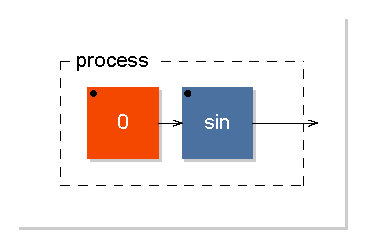
\includegraphics[]{CAPITOLI/0700/CODES/0701-seno-svg/process}
  \caption[]{Sine function. Faust Diagram.}
  \label{fdsine}
\end{figure}

\lstinputlisting{CAPITOLI/0700/CODES/0701-seno.dsp}

Questi sono i primi 5 campioni prodotti dalla formula $sin(0)$:

\lstinputlisting{CAPITOLI/0700/CODES/0701-seno.txt}

\lstinputlisting{CAPITOLI/0700/CODES/0702-senopi2.dsp}

Questi sono i primi 5 campioni prodotti dalla formula $sin(\pi/2)$:

\lstinputlisting{CAPITOLI/0700/CODES/0702-senopi2.txt}

questi i campioni

\lstinputlisting{CAPITOLI/0700/CODES/0703-senovariopi.txt}



%!TEX TS-program = xelatex
%!TEX encoding = UTF-8 Unicode
% !TEX root = ../metm.tex

\chapter{IL REPERTORIO}
\startcontents[chapters]
\printcontents[chapters]{}{1}{}

ciao\footcite[\emph{idem}]{prieberg:mexm}

Agamben \index[names]{Agamben, Giorgio}

\section{Luigi Nono}

NONO, Luigi (Venezia, 29.1.1924 – Venezia, 8.5.1990)

Nato il 29 gennaio 1924 a Venezia, primogenito di Mario Nono e Maria Manetti. Nono ebbe già nell’ambito familiare i primi stimoli per la sua formazione artistica e culturale: il nonno paterno, Luigi Nono, era un noto pittore della scuola veneziana di fine Ottocento; il prozio Urbano (fratello del pittore) uno scultore; la nonna materna, discendente dell’antica famiglia veneziana Priuli Bon, si dilettava col pianoforte e col canto spaziando dalla musica del passato alla produzione liederistica più recente (Nono ricorderà con stupore di aver rinvenuto tra i suoi spartiti una delle prime edizioni degli Italienische Lieder di Hugo Wolf accanto al Montezuma di Sacchini; Nono 1987, p. 480). La madre e il padre, di professione ingegnere, erano pianisti dilettanti che amavano cimentarsi con brani di repertorio (tra questi, il Boris Godunov di Modest Musorsgkij, spesso ricordato tra i primi ascolti nella sua fanciullezza; ibid.). Frequentatori assidui del Teatro La Fenice e di varie rassegne concertistiche, Mario e Maria Nono erano inseriti nei circoli culturali e musicali della migliore società veneziana. Grazie alla fornita discoteca del padre, Nono poté conoscere presto la musica di Beethoven, Wagner, Mahler nelle prime incisioni di direttori quali Toscanini o Mengelberg. Di non minore importanza furono le prime erratiche letture condotte sui libri della imponente biblioteca paterna (oggi in parte conservati nel lascito del compositore), dalle prime traduzioni italiane di poeti e scrittori russi, ai romanzieri americani pubblicati all’epoca da Einaudi, a Pavese, Gogol’, Rilke e vari altri autori che riaffioreranno nel corso degli anni tra le selezioni testuali delle proprie opere. In questa sfaccettata e privilegiata realtà domestica è possibile ravvisare l’origine di quella che diventerà una cifra caratteristica dell’universo artistico noniano, proiettato verso un’idea (e una pratica) della musica intesa come un’arte senza frontiere che può trovare ispirazione e fondamento in varie manifestazioni artistiche e scientifiche (pittura, architettura, letteratura, poesia, filosofia ecc.) delle diverse epoche storiche.

Intorno ai dodici anni Nono intraprese lo studio del pianoforte con una docente privata amica della madre (la signora Alessandri) e, fin da ragazzo, cominciò ad assistere agli spettacoli della Fenice e del Festival internazionale di musica contemporanea della Biennale di Venezia. Svolse i suoi studi presso il Ginnasio-Liceo classico «Marco Polo» di Venezia dove conseguì la maturità nel 1942. Nello stesso anno, per assecondare i desideri del padre, preoccupato delle incertezze della professione musicale, Nono si iscrisse alla Facoltà di Giurisprudenza dell’Università di Padova. Sempre nel 1942 egli conobbe il giovane pittore Emilio Vedova e intrecciò con lui un’amicizia che, rafforzatasi nel tempo anche grazie a varie collaborazioni artistiche, durò a fasi alterne fino alla morte del compositore.

La formazione scolastica e musicale di Nono si svolse negli anni cruciali del secondo conflitto mondiale e dell’immediato dopoguerra, in un clima familiare e intellettuale di stampo tradizionale e borghese ma perlopiù ostile al fascismo. Per motivi di salute egli fu dispensato dal servizio militare e non partecipò attivamente né alla guerra né alle successive fasi della Resistenza. Nono privilegiò nondimeno in quegli anni il contatto con giovani socialisti veneziani e personalità dell’opposizione locale, coltivando ideali politici e culturali non allineati con il regime.

Nel 1941, all’età di 17 anni, il padre gli procurò un incontro con una delle maggiori personalità musicali del tempo, Gian Francesco Malipiero, compositore che gli «aprì tutti gli orizzonti della musica» (Nono 1961, p. 3). Per qualche anno Nono seguì come studente esterno i suoi corsi di Composizione presso il Conservatorio di musica Benedetto Marcello di Venezia; dal 1943, dopo il ritiro di Malipiero dall’insegnamento di composizione, continuò a frequentare sempre da esterno la classe di contrappunto e fuga di Raffaele Cumar (ex allievo di Malipiero e Dallapiccola), approfondendo contemporaneamente in privato lo studio del pianoforte con Gino Gorini. In un periodo segnato culturalmente da una progressiva chiusura verso le esperienze d’avanguardia sviluppatesi in Europa dagli inizi del XX secolo, gli orizzonti aperti da Malipiero riguardavano lo studio di Monteverdi e della grande tradizione rinascimentale italiana (polifonica e madrigalistica), dei trattati teorici di Zarlino, Gaffurio e Vicentino, nonché la scoperta della musica di Arnold Schönberg, Anton Webern e Béla Bartók. Per la sua indole curiosa e irrequieta, Nono non riuscì mai ad adattarsi a piani di studio imposti e, ben presto, cominciò a nutrire una vera avversione per vincoli formativi legati a programmi ministeriali reputati noiosi e spesso inutili. Dopo il conseguimento del compimento inferiore e medio di composizione – sostenuti rispettivamente nel 1947 e 1949 presso il Conservatorio «Benedetto Marcello» – egli non reputò necessario coronare la sua formazione musicale con il diploma.

Nel 1946, grazie a Malipiero, Nono entrò in contatto con il giovane compositore e direttore d’orchestra veneziano Bruno Maderna, di soli quattro anni più anziano, già noto per il suo passato di fanciullo prodigio. All’incirca nello stesso periodo conobbe inoltre Luigi Dallapiccola, tra i musicisti più stimati e punto di riferimento per molti giovani della sua generazione. Delle prove compositive portate a termine prima del fondamentale incontro con Maderna resta solo la labile traccia di un ricordo (Nono 1979-80): nel 1945, durante la frequentazione di Malipiero – e influenzato anche dai suoi lunghi discorsi sulla musica del XV e XVI secolo –, Nono compose La discesa di Cristo agli inferi, brano (in seguito smarrito) forgiato sul modello delle sacre rappresentazioni e ispirato a un linguaggio di stampo monteverdiano (ivi, p. 242). Lo stimolo per il primo decisivo mutamento di rotta, dopo circa otto anni di studi musicali reputati parziali e insufficienti, sembrerebbe esser stato fornito proprio da un parere critico di Dallapiccola sulla partitura de La discesa di Cristo agli inferi, speditagli dal giovane compositore su suggerimento di Malipiero: «capisco che lei ha qui dentro nel cuore molto da esprimere, soltanto deve studiare ancora molto per poterlo esprimere» (ibid.). Queste parole costituirono per Nono una spinta a ricominciare gli studi musicali pressoché da zero in un nuovo periodo di apprendistato con Maderna. Conclusi gli studi universitari – coronati nel 1947 da una laurea in giurisprudenza con una tesi sul concetto giuridico dell’exceptio veritatis – egli poté dedicarsi solo alla musica e indirizzare il suo apprendistato verso un sentiero di conoscenza autonomo e responsabile, condotto al di fuori di ogni istituzione scolastica o accademica. (Di questo periodo 1946-47 non sono note composizioni al di fuori di un progetto vocale su liriche tratte da L’allegria di Giuseppe Ungaretti, poeta da tempo amato e ammirato.)

L’incontro con Maderna segnò in modo indelebile lo sviluppo musicale e umano di Nono, che riconobbe fino alla fine all’amico il ruolo di primo vero e grande maestro di vita.

Durante lunghe giornate trascorse tra l’abitazione di Maderna e la Biblioteca Marciana di Venezia, Nono approfondì – insieme ad altri giovani raccolti intorno al giovane maestro (Romolo Grano, Gastone Fabris e Renzo Dall’Oglio tra questi) – lo studio della musica del XV-XVI secolo, dall’ars antiqua all’ars nova francese, dai fiamminghi alla polifonia rinascimentale italiana, in un continuo confronto tra teoria e pratica. Tra gli autori più amati e analizzati: Guillaume de Machaut, John Dunstable, Johannes Ockeghem, Josquin Desprès, Adrian Willaert, Andrea e Giovanni Gabrieli, spesso trascritti a partire dall’Odhecaton di Ottaviano Petrucci. L’analisi di questo periodo storico divenne – tra la fine degli anni Quaranta e l’inizio del decennio successivo – lo stimolo per un’indagine comparata dei vari processi compositivi nella storia: data la comprensione di una tecnica musicale, il fine era scoprirne la funzione in relazione al momento storico, ricercandone nuove possibili trasformazioni o applicazioni nella musica delle epoche successive fino alla contemporaneità. Fondamentale importanza assunse per Nono l’analisi del rapporto tra lo stato del materiale, la sua elaborazione e l’epoca di produzione: fu grazie a questa peculiare ricerca che il compositore maturò la convinzione – in seguito mai abbandonata – che il linguaggio artistico deve svilupparsi di pari passo con i grandi movimenti politici e sociali del tempo, arrivando a essere una possibilità (o un mezzo) per poter intervenire all’interno di essi. Conoscere la musica del passato divenne, nel cenacolo maderniano, un mezzo per conoscere e impegnarsi responsabilmente nel proprio presente.


Fu sempre Maderna a far scoprire a Nono il manuale di tecnica compositiva di Hindemith (Unterweisung im Tonsatz, 1a ed. 1937) e, con esso, a suggergli – prima del comune approdo alla scrittura seriale – l’esistenza di soluzioni concrete e alternative nei confronti di un linguaggio armonico in crisi ormai da decenni. Nel 1948, ancora su suggerimento di Malipiero, Nono frequentò insieme a Maderna un corso internazionale di direzione d’orchestra tenuto a Venezia da Hermann Scherchen. Questo nuovo importante incontro segnò l’inizio di un lungo sodalizio (culturale e umano) tra i due giovani compositori e l’anziano direttore che, per circa cinque anni, divenne il loro fondamentale punto di riferimento. Nono cominciò a seguire Scherchen durante i suoi concerti, a soggiornare per lunghi periodi presso di lui (a Zurigo, Rapallo, Gravesano), e a collaborare dapprima come copista, poi come autore, con la sua casa editrice Ars Viva Verlag (acquisita negli anni Cinquanta dalla B. Schott’s Söhne di Magonza). Grazie a Scherchen, attraverso le sue esecuzioni e i suoi racconti, Nono entrò idealmente in stretto contatto con le esperienze – musicali e non – vissute dal direttore in Germania fin dal 1912, dalle prime esecuzioni assolute degli amati Schönberg e Webern alla realtà sociale e culturale tedesca precedente all’avvento del nazismo. Tra il 1948 e il 1949, su impulso di Scherchen Nono compose le Due liriche greche (inedite, formate da La stella mattutina e Ai Dioscuri, su testi rispettivamente di Ione di Ceo e Alceo nella traduzione italiana di Salvatore Quasimodo), dichiaratamente ispirate ai Canti di prigionia di Dallapiccola. Sempre dall’anziano direttore ricevette ulteriori stimoli allo studio della musica di Bach, Beethoven, Schumann e, soprattutto, del metodo dodecafonico, approfondito grazie all’analisi dei differenti approcci di Schönberg, Webern e Dallapiccola.

Nel 1950, su segnalazione di Scherchen e Maderna, Nono frequentò per la prima volta gli Internationale Ferienkurse für Neue Musik di Darmstadt – corsi estivi di musica contemporanea, fondamentale punto di incontro e di confronto per i giovani musicisti della generazione postbellica – debuttando sulla scena internazionale con il suo primo brano per orchestra, le Variazioni canoniche sulla serie dell’op. 41 di Arnold Schönberg (1949-50). Diretta da Scherchen, l’opera fu accolta in modo non unanime ma, al contempo, rivelò la centralità del giovane compositore nel contesto delle problematiche e delle discussioni dell’avanguardia musicale coeva. L’esperienza di Darmstadt – luogo frequentato ininterrottamente per dieci anni (dal 1957 come docente) – costituì un momento di fondamentale importanza nella sua evoluzione artistica, umana e politica. Fu qui che Nono ebbe modo di approfondire ulteriormente la musica dodecafonica e, in particolare, quella di Schönberg; di conoscere Edgard Varèse (tra gli estimatori delle Variazioni canoniche in occasione della contrastata prima esecuzione) e approcciarsi alla sua musica visionaria che tanta importanza ebbe nelle successive evoluzioni del pensiero sonoro noniano. In questa sede egli instaurò importanti rapporti – alimentati dalla consentaneità così come dal dissenso – con vari musicisti europei ed extraeuropei tra cui Karlheinz Stockhausen, Pierre Boulez, Henri Pousseur, John Cage. Soprattutto, fu a Darmstadt che si ebbero le prime esecuzioni assolute di alcune tra le più importanti pagine degli anni Cinquanta: alle già citate Variazioni canoniche seguirono infatti Polifonica-Monodia-Ritmica (1951), l’Epitaffio per Federico García Lorca I. España en el corazón (1952), La victoire de Guernica (1954), Incontri (1955), Cori di Didone (1958) e, ancora, Composizione per orchestra n. 2: Diario Polacco ’58 (1959).

Sono, queste, le opere che rivelarono Nono come uno dei maggiori rappresentanti dell’avanguardia europea e del linguaggio seriale, insieme a Stockhausen e Boulez. Da questi stessi compositori, e dall’ambiente dei Ferienkurse, egli prese nondimeno le distanze in modo dichiarato nel 1959, allorché con la conferenza Geschichte und Gegenwart in der Musik von heute (reso in italiano come Presenza storica nella musica d’oggi) polemizzò apertamente contro alcuni rappresentati dell’avanguardia e con la cosiddetta «Scuola di Darmstadt» (espressione da lui stesso coniata, cfr. Nono 1957, p. 34), denunciandone incoerenze e aporie. Dopo anni in cui gli stimoli si erano intrecciati a costruttivi conflitti, questo intervento sancì una prima frattura con il luogo e con alcuni dei suoi rappresentanti (primo tra tutti Stockhausen). L’inconciliabilità delle posizioni riguardava tanto alcune derive iperdeterministiche dei seguaci della serialità integrale e il loro rifarsi a modelli ricavati dalle scienze naturali, quanto esperienze di segno opposto riconducibili all’alea e all’indeterminazione (Cage fu apertamente nominato come pars pro toto). Entrambe le tendenze furono additate da Nono come fuga dalla storia e sintomo di una irresponsabile volontà di evitare chiare prese di posizione nei confronti di problematiche artistiche del proprio presente. La rottura, definitiva, fu quindi sancita nel 1960 con la nuova conferenza Text – Musik – Gesang (pubblicata in italiano come Testo – musica – canto), dove la distanza dalle posizioni di Stockhausen e da un’ortodossia seriale ormai vissuta come gabbia assunse infine i toni dell’aperto attacco.

Nel 1954, in occasione della prima rappresentazione del Moses und Aron di Schönberg, Nono conobbe ad Amburgo la figlia del grande compositore austriaco, Nuria, che sposò l’anno successivo. Dal matrimonio nacquero due figlie, Silvia (1959) e Serena Bastiana (1964). Tra la fine del 1958 e gli inizi del 1960 Nono compì inoltre la sua unica (nonché atipica) esperienza di docente con Helmut Lachenmann che, per lunghi periodi, soggiornò a Venezia collaborando con Nono alla formulazione tedesca delle due menzionate conferenze tenute ai Ferienkurse di Darmstadt.

Negli stessi anni Cinquanta furono di grande importanza la scoperta o l’approfondimento delle esperienze politiche e culturali d’oltralpe, della Rivoluzione sovietica e della cultura della Repubblica di Weimar, delle avanguardie storiche russe e tedesche e delle innovazioni in campo teatrale di Vsevolod Mejerchol’d, Vladimir Majakovskij, Erwin Piscator. Sollecitazioni, queste, che vennero ad aggiungersi al parallelo entusiasmo per la rivelazione dell’insegnamento di Antonio Gramsci, del pensiero filosofico di Jean-Paul Sartre, di una produzione poetica ancorata alle problematiche del proprio tempo e rappresentata da autori quali Federico García Lorca, Pablo Neruda, Paul Éluard, Cesare Pavese, Giuseppe Ungaretti.

È soprattutto da questi scrittori che Nono seleziona i testi per le proprie opere vocali degli anni Cinquanta, decennio al cui centro campeggia uno dei suoi capolavori, Il canto sospeso (1955-56), basato su lettere di condannati a morte della Resistenza europea. Abbandonato l’uso di materiali ritmici preesistenti – proprio alle sue pagine composte tra il 1950 e il 1953 – e approfondita quella personale elaborazione della tecnica seriale già avviata in campo strumentale con Canti per 13 (1955), Nono perfezionò le proprie conquiste compositive nel campo della vocalità: con Il canto sospeso approdò a una nuova pratica basata su una peculiare tecnica di frammentazione del testo, enunciato nelle sue componenti vocaliche o fonetiche in successione tra le singole voci o simultaneamente, come blocco o aggregato sonoro.

Come testimoniano anche vari scritti teorici redatti nel corso degli anni Cinquanta, è in questo periodo che si rafforzarono in Nono le proprie idee sulla capacità comunicativa della musica e sulla necessità di poter e dover esprimere attraverso la propria arte le sfaccettate contraddizioni del proprio tempo. Gradualmente la selezione dei testi fu sempre più orientata verso temi politicamente impegnati tratti dall’attualità storico-sociale del presente o dell’immediato passato. Questo aspetto si rivelò in tutta la sua evidenza a partire dall’azione scenica Intolleranza 1960 (1960-61) – opera in cui si concretizzarono per la prima volta alcune idee su un “nuovo teatro musicale” maturate nel corso degli anni Cinquanta – e giunse al culmine nella prima metà degli anni Settanta con la seconda azione composta per le scene, Al gran sole carico d’amore (1972-74, rev. 1977).

L’esperienza teatrale di Nono si era inizialmente nutrita di un sentimento di rifiuto – comune a diversi giovani compositori dell’avanguardia post-bellica – nei confronti dei modelli operistici fin de siècle, negazione in cui si rispecchiava un aperto dissenso verso l’organizzazione della società borghese. Fin dai primi progetti drammaturgici tracciati nel corso degli anni Cinquanta – tra i quali vari soggetti mai realizzati su testi di John Steinbeck, Anna Seghers e Anna Frank –, il teatro fu inteso come un luogo in cui temi attuali avrebbero dovuto essere rappresentati con mezzi espressivi e scenotecnici altrettanto originali. La ricerca di Nono in ambito scenico si concentrò in quegli anni sulle esperienze teatrali (soprattutto non musicali) del primo ventennio del Novecento. Come era avvenuto con lo studio della musica del passato condotto sotto la guida di Maderna, anche l’approdo al teatro musicale fu edificato sulla base di un’indagine storica atta ad approfondire tutte quelle esperienze artistiche che, proprio per essere state condannate o represse da regimi diversi, apparivano come modelli ancora potenzialmente attuali. Le letture condotte da Nono nel corso degli anni Cinquanta sul tema «teatro» furono numerose e discontinue: dalle esperienze di Gropius e del Bauhaus commentate da Giulio Carlo Argan (Einaudi 1951) alla storia del teatro di Baty-Chavance (Einaudi 1951), dai libri sul teatro russo e tedesco dei primi anni del Novecento (tra cui il fondamentale testo sul teatro politico di Piscator, 1929) a volumi su e di Majakovskij, Brecht, ecc. L’analisi parallela dei suoi approfondimenti teorici e dei suoi primi progetti drammaturgici sembra suggerire che già dai primi mesi del 1952 il compositore avesse posto le basi di quella personale riflessione sulle implicazioni tecniche e sulle possibilità di una funzione politica del teatro che, nel 1960-61, condusse alla prima azione scenica, Intolleranza 1960 (su testo proprio, rielaborato dal compositore a partire da un’idea di Angelo Maria Ripellino, con passi tratti da Alleg, Brecht, Éluard, Fučik, Majakovskij, Sartre e dallo stesso Ripellino; realizzato scenicamente con la collaborazione di Josef Svoboda ed Emilio Vedova). Soprattutto a causa dei suoi contenuti politici, in occasione della sua prima messa in scena (Venezia, 1961) l’opera scatenò violente contestazioni in sala e, nel panorama musicale dell’epoca, costituì un vero evento che divise il giudizio di pubblico e critica. Pressoché ignorata nella sua prima ricezione fu invece la portata innovativa dei suoi contenuti musicali: Intolleranza 1960 si poneva infatti come un’opera spartiacque, al contempo momento di sintesi e laboratorio sperimentale in cui tecniche ormai acquisite si affiancavano a nuove procedure compositive proiettate verso il futuro. In essa convergevano tutte le maggiori conquiste tecnico-linguistiche che avevano inaugurato gli anni Sessanta. Tra queste, la nuova tecnica vocale della “linea unica” sperimentata nei brani a cappella Sarà dolce tacere e «Ha venido». Canciones para Silvia (entrambe del 1960) e, tra le conquiste più importanti in prospettiva futura, l’uso del nastro magnetico e degli strumenti di produzione elettroacustica del suono. Sempre al 1960 data infatti la prima composizione elettronica di Nono, Omaggio a Emilio Vedova, realizzata presso lo Studio di Fonologia della RAI di Milano, laboratorio elettronico dove per diciannove anni, fino al 1979, egli produsse tutte le sue opere per/con nastro magnetico. A partire da questo momento, l’esperienza elettronica divenne una costante dell’itinerario creativo di Nono, che usò il mezzo tecnologico come nuova frontiera per esprimersi artisticamente in modo sempre più libero e immediato, sperimentando di volta in volta soluzioni sonore e spaziali non ottenibili con una liuteria tradizionale e, soprattutto, non più classificabili in generi musicali codificati. Fu anche grazie all’elettronica che Nono dismise gradualmente sistemi compositivi rigidamente organizzati, quali griglie seriali e di regolazione statistica dei parametri musicali (proprie alle composizioni degli anni Cinquanta), privilegiando sempre più l’organizzazione degli eventi sonori in strutture locali e l’elemento intervallare in luogo di quello ritmico. Svincolata da serie e da un preordinato controllo delle altezze, la scelta degli intervalli divenne per Nono sempre più “intuitiva”, definita localmente e proiettata verso la giustapposizione o sovrapposizione di superfici di suono complesse (blocchi, fasce, linee, ecc.).

L’impegno politico, i temi di conflittualità e denuncia sociale, il rifiuto della psicologia individuale a favore dell’amplificazione collettiva del dramma – tutti elementi propri all’orizzonte testuale di Intolleranza 1960 – divennero una costante nel corso degli anni Sessanta e Settanta, nel corso dei quali il concetto di impegno acquisì per Nono il valore di «imperativo morale» (J.P. Sartre) da affiancare a quello estetico. Il rapporto tra arte e attualità divenne sempre più intrecciato e profondo: ogni brano, realizzato o solo progettato, era concepito come un mezzo per partecipare attivamente, e con i propri strumenti specifici, a un più ampio processo di trasformazione della realtà sociale.

Spogliato il termine “ideologia” dell’accezione negativa propria della concettualizzazione marxiana, Nono ricondusse questa categoria di pensiero al significato gramsciano di “idea del mondo” esaltandone le caratteristiche di “strumento di verità” e di “funzione sociale” inscindibili dal messaggio artistico. A queste funzioni l’autore collegava senza mediazione lo sviluppo di un proprio peculiare linguaggio musicale, di una tecnica compositiva intesa anche come mezzo per arrivare a una testimonianza eticamente consapevole del proprio presente. Questo bisogno di attualità coinvolgeva il doppio piano del contenuto e della forma, binomio che caratterizzò, fin dagli esordi di Nono, il rapporto tra creazione e impegno. Ne La fabbrica illuminata (1964), per esempio, una voce dal vivo interagisce con se stessa preregistrata su nastro magnetico e vari materiali sonori (rumori, voci di operai ecc.), registrati dal vivo nella fabbrica dell’Italsider di Genova Cornigliano quindi elaborati elettronicamente in Studio. La denuncia, implicita nei testi documentari rielaborati da Giuliano Scabia sulla condizione operaia, è bilanciata in chiusura da una ferma fiducia nell’amore e nel futuro, in un chiaroscuro dramma-speranza caratteristico di molte opere vocali di Nono. Impegnate in una dimensione internazionale e terzomondista sono le successive A floresta é jovem e cheja de vida (1965-66), su testi documentari curati da Giovanni Pirelli, e Y entonces comprendió (1969-70), su testi di Carlos Franqui ed Ernesto “Che” Guevara. In queste opere l’alternanza tra voci dal vivo e preregistrate è ulteriormente sperimentata ed elaborata; si radicalizzano inoltre alcuni aspetti di prassi compositiva (intimamente legati a problematiche di prassi esecutiva) determinanti nella poetica musicale noniana degli anni Settanta-Ottanta. A partire da opere come La fabbrica illuminata o A floresta é jovem e cheja de vida il processo creativo di Nono venne infatti progressivamente a definirsi sempre a più stretto contatto con interpreti specifici, selezionati per le loro peculiarità timbriche ed espressive (in questa fase si ricordano, tra gli altri, i nomi di Carla Henius, Kadigia Bove, Elena Vicini). Grazie al lavoro condotto con gli interpreti in fase compositiva, Nono cominciò a non sentire più l’esigenza di fissare in un modo unico e definitivo la sua volontà autoriale in un’edizione a stampa (come nel caso di A floresta, ricostruita ed edita post mortem nel 1998). Soggetta a variabili ambientali, di proiezione spaziale del suono in sala, microfoniche ecc., l’opera cominciò ad essere intesa come prodotto di un processo in continuo divenire, spesso lasciata allo stadio di istruzione, appunto, progetto o schizzo e definita in forma conchiusa nelle sole direttive date all’interprete (la cui memoria spesso poteva coincidere in parte o in toto con il testo dell’opera). Anche laddove edite, come nel caso di Y entonces o della successiva Como una ola de fuerza y luz (1971-72, su testo di Julio Huasi), le creazioni venivano comunque definite gradualmente grazie a un lavoro condotto anche insieme agli interpreti (vocali, strumentali o addetti alla regia del suono) e orientato sempre più verso una pratica esecutiva del tutto atipica rispetto alle consuetudini tradizionali.

Ogni scelta testuale e/o performativa operata in questi anni testimonia della incessante volontà di Nono di intendere la musica come un mezzo di lotta, politica e sociale, per arrivare a denunciare ingiustizie e assurdità del presente. Nella biografia artistica e umana di Nono, la problematica relativa al concetto di impegno è stata (ed è ancora oggi) uno degli aspetti più complessi, dibattuti e, a seconda delle letture più o meno di parte, soggetto ad equivoci. Iscritto al Partito Comunista Italiano dal 1952 (quindi dal marzo del 1975 membro del Comitato Centrale), amico di esponenti e vertici del partito o critici marxisti militanti (Luigi Pestalozza tra questi), Nono non venne mai meno a un’ideale di artista d’avanguardia engagé, e questo anche quando – nelle ultime fasi della sua vita – l’impegno e la denuncia assunsero forme meno dirette. Il periodo più fecondo sul piano politico fu quello degli anni Sessanta-Settanta, in cui spesso i dati artistici giunsero a coincidere con quelli biografici (si pensi ai vari viaggi condotti nei paesi dell’Est a partire dal 1958, nell’URSS nel 1963 e negli anni Settanta, negli USA nel 1965 e nel 1979, nei paesi dell’America Latina – dal Cile al Perù a Cuba – a partire dal 1967; e ancora al confronto con la teoria e con la prassi del marxismo internazionale, la partecipazione alle lotte operaie degli anni Sessanta e ai movimenti studenteschi del 1968 ecc.). La militanza politica – esplicitamente dichiarata nelle scelte di carattere etico, sociale e artistico – divenne in questa fase inscindibile da quella di musicista alla continua ricerca di nuove soluzioni sonore. Proprio sul doppio terreno della politicizzazione delle opere e di un uso “rivoluzionario” dell’elettronica si consumò, nel 1964, la rottura con il suo primo editore storico, l’Ars Viva Verlag (Schott), e il conseguente passaggio alla Ricordi. Nel corso degli anni Sessanta-Settanta più volte Nono ebbe a parlare della propria musica come del prodotto di un’unione tra tecnica e ideologia, affermando a chiare lettere la propria “necessità” di declinare la musica al presente: «Sicuramente una partitura può causare una rivoluzione così poco come un quadro, una poesia o un libro; ma una musica può esattamente come un quadro, una poesia o un libro dare nota dello stato desolato della società, può contribuire, può fondare consapevolezza se le sue qualità tecniche si mantengono allo stesso livello di quelle ideologiche» (Nono 1969, p. 26). Questa e simili testimonianze contenute in altri testi redatti negli anni Sessanta (quali Il musicista nella fabbrica, 1966, o il testo di presentazione per Contrappunto dialettico alla mente, 1968) si sono rivelate spesso fuorvianti in sede critica, dove si è spesso dato più peso alle «qualità ideologiche» che alla portata innovativa e al valore artistico della sua musica.

Leggendo il dato in retrospettiva, la relazione tra arte e ideologia affonda le radici nello stesso apprendistato condotto con l’amico-mentore Maderna alla fine degli anni Quaranta e costituisce una tra le premesse creative della sua opera di esordio, di quelle Variazioni canoniche sulla serie dell’op. 41 di Arnold Schönberg intese come «conseguenza dei miei primi studi dei canoni enigmatici ma […] anche una scelta ideologica» (Nono 1979-80, p. 242). Nella fase più dichiaratamente engagée dell’evoluzione di Nono, il coinvolgimento politico procurò indiscutibili impulsi alla creazione: «sempre – scrisse presentando la Composizione per orchestra n. 2 – Diario polacco ’58, composta a seguito del suo primo viaggio in Polonia – la genesi di un mio lavoro si basa su una provocazione umana: un avvenimento, una esperienza, un testo della nostra vita provoca il mio istinto e la mia conoscenza a dare la testimonianza di me musicista-uomo» (Nono 1960, p. 433), parole applicabili anche alle ultime fasi del suo percorso artistico.

Queste «provocazioni», o stimoli, sono spesso palesi e verificabili nelle scelte dei materiali e dei collaboratori. Per le fonti testuali, gli anni Sessanta-Settanta sono segnati dalla ricerca di testi tratti da autori o soggetti storici che fossero al contempo simboli di lotta, di forza, di speranza e di sacrificio per la collettività (Karl Marx, “Che” Guevara, Rosa Luxemburg, Bertolt Brecht, Fidel Castro, Tania Bunke, ecc.). Per le fonti sonore, Nono fece spesso ricorso in questi anni a suoni concreti delle realtà operaie o di rivolta, fissati nelle sue opere con/per nastro magnetico, in cui violenza umana e sonora si intrecciano talora indelebilmente (come ne La fabbrica illuminata, in A floresta o in Non consumiamo Marx, seconda parte del dittico Musica-Manifesto n. 1, 1969). Sul fronte delle collaborazioni, si pensi a quella con Piscator nel 1965, con la realizzazione delle musiche elettroniche per lo spettacolo teatrale Die Ermittlung [L’istruttoria] di Peter Weiss; al sodalizio umano e artistico che lo legò a Claudio Abbado e Maurizio Pollini, conosciuti rispettivamente nel 1965 e nel 1966, interpreti legati indissolubilmente alla genesi di alcune tra le sue pagine più importanti (“su” e “per” Pollini fu ideata la parte pianistica di Como una ola de fuerza y luz, 1971-72 e …..sofferte onde serene…, 1976, laddove Abbado sarà sul podio delle prime assolute di Come una ola, Al gran sole carico d’amore, Prometeo); si pensi ancora al lavoro con il Living Theatre nel 1966 per il nastro di A floresta o, ancora, al lavoro collettivo con il regista e lo scenografo del teatro Taganka di Mosca (Jurij Ljubimov e David Borovskij) per Al gran sole carico d’amore. Questa seconda azione scenica, dedicata alle lotte di liberazione di tutto il mondo, segnò l’acme del periodo apertamente politico di Nono: dalla Comune di Parigi alla rivoluzione russa del 1905 a quella cubana ecc., varie sommosse per la libertà furono lette da Nono attraverso il ruolo assunto al loro interno dalle donne, simbolo di speranza forza e amore. Comporre, fare e diffondere musica, diventò dichiaratamente per il compositore un momento di sintesi dialettica tra arte e vita, vista come la sola maniera per «realizzarsi compiutamente» (Nono 1963, 144). Nei concetti di impegno e responsabilità sembra riaffiorare in Nono – apertamente negli anni centrali della sua “lotta” artistica, in modo più sotterraneo negli Ottanta – l’eco dell’insegnamento di Piscator, il cui volume Das politische Theater (del 1929, edito in Italia da Einaudi nel 1960) fu una lettura determinante per Nono nei primi anni Cinquanta, allorché il compositore prendeva gradualmente coscienza del fatto che «la sintesi di arte e politica significa suprema responsabilità, significa mettere al servizio delle supreme mete umane tutti i propri mezzi e dunque anche l’arte» (Piscator, Il teatro politico, Torino 1960, p. 48).

Ma, all’interno di una parabola compositiva quasi quarantennale che lo portò dalla serialità alla musica elettronica ai live electronics, per impegno bisogna intendere anche una visione “responsabile” della ricerca implicita in ogni nuova composizione e nella messa a punto di un linguaggio innovativo la cui rivoluzione è nel risultato sonoro. In questa prospettiva va ridimensionata, o addirittura respinta, l’idea di una presunta fase “a-politica” attribuita al Nono degli anni Ottanta: l’arte vissuta come responsabilità e impegno soggettivo (che lega l’autore, l’esecutore e l’ascoltatore) è una costante che accomuna l’intero itinerario artistico del compositore e che esula da messaggi politici, palesi o latenti.

Per la comunicazione dei propri messaggi sonori, Nono percepì come profondamente inadeguati tanto i tradizionali luoghi di produzione e diffusione musicale, quanto le procedure esecutive ad essi sottesi. Nel corso degli anni Sessanta-Settanta il lavoro si proiettò sempre più verso una dimensione collettiva; le fabbriche divennero sale da concerto; la ricerca di un nuovo teatro musicale fu equiparata tout court a una condanna delle tradizionali consuetudini di ascolto e fruizione degli spettacoli. Più che le istituzioni, furono piuttosto le forme e le consuetudini sedimentate in quelle istituzioni (culturali, concertistiche, sociali) ad essere considerate superate e discusse costantemente. Lo stesso concetto di “impegno” arrivò ad essere declinato anche nell’uso dello spazio. Nei progetti e nelle opere sceniche compiute – da Intolleranza 1960 alla «tragedia dell’ascolto» Prometeo (1984, rev. 1985) – divenne sempre più radicale la volontà di abbattere la tradizionale separazione tra scena e pubblico, vista da Nono come retaggio di una rappresentazione rituale e “antidemocratica” con «i fedeli che assistono e l’officiante che celebra» (Nono 1962, p. 122). Innovativa, in questo caso, non era l’idea in sé, già largamente dibattuta e sperimentata soprattutto in campo non musicale dalle avanguardie russe, nelle sperimentazioni di Gropius o nel teatro di Piscator (laddove in campo musicale vanno quantomeno ricordati alcuni esperimenti quali Passaggio di Luciano Berio, 1962).

Innovativa è, piuttosto, la dimensione sonora e visiva che Nono intendeva proiettare in uno spazio senza barriere, fisiche o ideali, di fruizione artistica. Lo “spazio” immaginato dal compositore – raggiunto negli anni Ottanta con la trasformazione, elaborazione e proiezione in tempo reale del suono consentita dai live electronics – era inteso come un ambiente in cui i rapporti spazio-temporali potessero infrangersi in una dimensione totale sia sul piano acustico (con la moltiplicazione e spazializzazione delle sorgenti sonore), sia su quello visivo (attraverso l’eliminazione della separazione tra scena e platea).

A metà degli anni Settanta, dopo la seconda importante tappa teatrale raggiunta con Al gran sole carico d’amore, intervenne nella vita di Nono una profonda crisi creativa amplificata dal doppio lutto che, a distanza di pochi mesi, lo colpì con la morte del padre (ottobre 1975) e della madre (gennaio 1976). Pochi anni dopo quegli eventi, così Nono rievocò quel particolare momento insieme ai cambiamenti umani e artistici che ne derivarono: «Subito dopo Al gran sole è venuto il silenzio, un silenzio inesprimibile: non avevo cioè i mezzi adatti ad esprimermi. Contemporaneamente è iniziato il mio rapporto di amicizia con Massimo Cacciari che pure conoscevo dal 1965. Ho sentito una necessità di studio non solo sul mio linguaggio musicale ma anche di analisi delle mie categorie mentali e ho ripreso a comporre con …..sofferte onde serene…, un lavoro che mi ha impegnato moltissimo» (Nono 1979-80, p. 245). Alle precedenti conquiste – quali la funzione prioritaria dell’interprete nel processo creativo, il ruolo delle tecnologie, ecc. – si affiancò una nuova tensione verso un’interiorizzazione del messaggio musicale e del concetto di impegno. Le principali caratteristiche dello stile che inaugura gli anni Ottanta – resosi manifesto a partire dal quartetto d’archi Fragmente-Stille, an Diotima, 1979-80 – sono il silenzio, la pausa, la giustapposizione di frammenti in cui pianissimi al limite dell’impercettibile si alternano a esplosioni sonore, il valore strutturale dello spazio.

Sebbene questi elementi abbiano portato alcuni critici ed esegeti a parlare di una “svolta” (memorabile l’articolo che nel 1988 Massimo Mila dedicò a quest’ultima fase noniana, intitolato appunto Nono, la svolta), o di repentine discontinuità nel percorso artistico noniano, è nondimeno da rilevare che tutti questi elementi erano già presenti in nuce (e altrimenti declinati) in diverse opere degli anni Cinquanta: silenzi e sonorità sulla soglia dell’inaudibile erano per esempio in Polifonica-Monodia-Ritmica, così come i chiaroscuri dinamici e le sonorità lacerate proprie di alcune opere degli anni Ottanta erano in Due espressioni per orchestra (1953), Il canto sospeso, La terra e la compagna (1957) o nei Cori di Didone. In aperta contraddizione con interpretazioni tecniche o stilistiche che procedono per decenni, nella totalità dell’arco creativo di Nono è possibile rintracciare il filo di uno sviluppo continuo, di un’incessante elaborazione di elementi messi al servizio di un’idea sonora immaginifica, confinante talvolta con l’utopia.

I mutamenti politici e sociali, la consapevolezza della progressiva perdita di un soggetto collettivo e dell’illusorietà di una rivoluzione sociale si palesano nelle scelte testuali delle opere degli anni Ottanta, in cui risulta evidente l’influsso dell’amico filosofo Massimo Cacciari. Friedrich Hölderlin, Rainer Maria Rilke, Robert Musil, la mistica ebraica, Walter Benjamin, Edmond Jabès, Giordano Bruno, Friedrich Nietzsche, il pensiero della tragedia e della mitologia greca: questi gli autori o testi rielaborati da Cacciari per Das atmende Klarsein (1981), Quando stanno morendo. Diario polacco n. 2 (1981), Guai ai gelidi mostri (1983) e per l’atipica opera Prometeo. A questi nuovi stimoli letterari si affiancarono le nuove risorse tecniche offerte dagli strumenti di trasformazione del suono in tempo reale (live electronics), sperimentate e approfondite in Germania presso l’Experimentalstudio der Heinrich-Strobel-Stiftung di Friburgo. Nono cominciò a frequentare questo nuovo laboratorio elettronico dal 1980 a seguito del suo addio allo Studio di Fonologia della RAI, ormai tecnologicamente vetusto, sancito dopo la messa a punto di Con Luigi Dallapiccola (1979), omaggio a una delle sue guide spirituali di gioventù e prima opera in cui i suoni – dismesso l’uso di nastri magnetici – sono trasformati in tempo reale.

Il pensiero sotteso alle creazioni dell’ultimo decennio – caratterizzate da un procedere per “tentativi” o “scelte”, e dalle costanti trasformazioni degli eventi sonori in sede di esecuzione – ricorda l’immagine dello scultore leonardiano, che «nel fare la sua opera fa per forza di braccia e di percussione a consumare il marmo, od altra pietra soverchia, ch’eccede la figura che dentro a quella si rinchiude» (Leonardo, Trattato della pittura, § «Differenza tra la pittura e la scoltura»). Questo procedere per sottrazione modellando il suono in tempo reale, spesso arricchito da nuove possibilità nate come reazioni ad errori tecnici, è evidente nel cammino che conduce al Prometeo, edificato sulle tappe preliminari di diversi brani intesi come “studi”: Das atmende Klarsein, Io, frammento dal Prometeo (1981), Quando stanno morendo. Diario polacco n. 2, Guai ai gelidi mostri. Sebbene Prometeo venga annoverato tra le opere teatrali di Nono, in esso si compie un’azione di totale scarnificazione dell’elemento scenico, del tutto dismesso, o narrativo: il “teatro”, l’azione, è nel suono, inteso come entità mobile, avulso da qualsivoglia apparato visivo e drammaturgicamente proiettato in uno spazio risonante edificato anche grazie alla struttura di legno in forma di “arca”, espressamente concepita da Renzo Piano per lo spazio della chiesa veneziana di S. Lorenzo (che ne ospitò la prima esecuzione assoluta nel 1984). Idealmente, il Prometeo può essere visto come l’approdo dei tentativi teatrali intrapresi all’indomani di Intolleranza 1960, proiettati verso un orizzonte sonoro in cui la vista lascia gradualmente il campo al puro ascolto. Sul piano dei contenuti testuali l’opera mirava invece non a una rilettura mitologica della figura di Prometeo quanto all’affermazione della sua portata “rivoluzionaria”, vista nella sua incessante ricerca di nuovi ordini che sovvertissero i precedenti: «in una parola, [del]la continuità prometeica senza fine» (Nono 1987, p. 559).

La ricerca di realtà sonore inaudite, tali da provocare non solo una differente maniera di “vivere” il suono (da parte di interpreti e fruitori) ma da richiedere anche diverse configurazioni degli spazi da concerto, è alla base dell’ultima produzione di Nono che, lontana dall’essere apolitica o disimpegnata, proietta l’ideale di un’arte tanto umana quanto impegnata nelle sfere interiori dell’“indicibile” (temi tra i più cari all’ultimo Nono, insieme a quello dell’“utopia”). All’indomani del Prometeo, conclusasi la collaborazione con Cacciari e tra soggiorni in Germania sempre più frequenti, Nono scrisse le sue opere orchestrali più visionarie: A Carlo Scarpa architetto, ai suoi infiniti possibili (1984), per orchestra a microintervalli; Caminantes… Ayacucho (1986-87) e «No hay caminos. Hay que caminar»… Andrei Tarkowskij (1987). Queste pagine per grande organico furono affiancate da brani con organico ridotto e trattamento del suono live electronics – tra queste i due omaggi a Boulez e Cacciari, A Pierre, dell’azzurro silenzio, inquietum (1985) e Risonanze erranti. Liederzyklus a Massimo Cacciari (1986) – e da brani solistici con o senza la trasformazione del suono in tempo reale: Post-Prae-Ludium per Donau (1988), La lontananza nostalgica utopica futura. Madrigale per più «caminantes» con Gidon Kremer (1988-89), scritta “sul” grande violinista citato nel titolo, e «Hay que caminar» sognando (1989), brano che chiude il catalogo noniano. Ciascuna di queste opere venne realizzata pressoché costantemente con singoli interpreti di fiducia – Roberto Fabbriciani, Ciro Scarponi, Giancarlo Schiaffini, Susanne Otto, Stefano Scodanibbio, Hans Peter Haller ecc. – spesso vicini al compositore anche nelle fasi preparatorie dell’opera in lunghe sedute di lavoro e studio presso il laboratorio elettronico di Friburgo, depositari di una volontà d’autore sempre più refrattaria ai limiti e margini di una scrittura musicale difficilmente codificabile in modo tradizionale.

Nei suoi ultimi anni di vita Nono intensificò i suoi rapporti con la Germania vivendone dall’interno le fasi che precedettero la caduta del Muro di Berlino. Altri viaggi decisivi per la genesi di alcune opere furono condotti in Spagna; fu proprio a Toledo, nel 1985, che lesse sul muro di un convento la parafrasi di un verso di Machado – «Caminantes: no hay caminos, hay que caminar» – fonte di ispirazione per il ciclo dei Caminantes che chiude il suo catalogo. Nel 1986-87 soggiornò per un lungo periodo a Berlino grazie a una borsa del DAAD (Deutscher Akademischer Austauschdienst, servizio tedesco per lo scambio accademico). Nel 1987-88 divenne membro del prestigioso istituto di ricerca Wissenschaftskolleg zu Berlin. Nel marzo 1990 vinse il Großer Kunstpreis Berlin, importante onorificenza annualmente conferita da una delle sei sezioni dell’Akademie der Künste a personalità di spicco in campo artistico. Ormai gravemente ammalato di una disfunzione epatica, Nono si spense a Venezia due mesi dopo, l’8 maggio 1990, nella sua dimora natale alle Zattere.

(Angela Ida De Benedictis, versione ampliata della voce Luigi Nono, Dizionario Biografico degli Italiani, Treccani.it L’enciclopedia italiana, Volume 78, 2013 / © Treccani. Per gentile concessione dell’editore e dell’autrice).


%!TEX TS-program = xelatex
%!TEX encoding = UTF-8 Unicode
% !TEX root = ../metm.tex

\chapter{LE FIGURE DELLA MUSICA}
\startcontents[chapters]
\printcontents[chapters]{}{1}{}

\begin{flushright}
		\textit{We think we're writing something to amuse, but \\
            we're actually saying something we desperately need to share. \\
            The real mystery is this strange need. \\
            Why can't we just hide it and shut up? \\
            Why do we have to blab? \\
            Why do human beings need to confess? \\
            Maybe if you don't have that secret confession, \\
            you don't have a poem - don't even have a story. \\
            Don't have a writer.} \\
            - Ted Hughes\footnote{Ted Hughes, \emph{The Art of Poetry No. 71}, \emph{The Paris Review}, n. 134 - 1995\\
						Pensiamo di scrivere qualcosa per intrattenere, ma | in realtà stiamo
						dicendo qualcosa che abbiamo disperatamente bisogno di condividere. |
						Il vero mistero è questo strano bisogno. | Perché non possiamo
						semplicemente nasconderlo e stare zitti? | Perché dobbiamo spifferare? |
						Perché gli esseri umani hanno bisogno di confessare? | Forse se non
						si ha quella confessione segreta, |	non si ha una poesia - non si
						ha nemmeno una storia. | Non si ha uno scrittore.}
\end{flushright}

\section{Compositore}

\emph{Chi è compositore oggi? Una persona che viene pagata per scrivere musica?
Una che produce dischi per i quali ha decine di sostenitori? Una persona che
insegna composizione? Una che è diplomata in composizione?}

La figura del compositore di musica è, oggi, un buon argomento di discussione e
\emph{deve} esserlo in ogni ambito di studi che possa presentare orizzonti compositivi.

Composizione è tecnica. Tecnica è regole. \emph{Composizione è regole?} Indispensabile
riflessione storica su questo punto è quella di Giorgio Nottoli\index{Nottoli, Giorgio} (1997) in
\emph{a proposito di musica contemporanea} pubblicato su \emph{Fisica nella Musica}
di Alberto Frova. In quel testo Nottoli\index{Nottoli, Giorgio} compone un ragionamento sulla composizione,
sull'essere compositore investendo inevitabilemente di responsabilità anche la
controparte, il fruitore, l'essere destinatario di quella che John Cage\index{Cage, John} definisce
\emph{lettera ad uno sconosciuto}: la composizone di un brano musicale.

Il testo si articola attorno ad un centro logico formato dal triangolo
\emph{regola-libertà-processo} che racchiude e protegge il cuore della composizione:
l'\emph{idea musicale}. Senza \emph{idea}, non c'è processo, né regole né
libertà d'azione. L'artista, il compositore, manipola l'\emph{idea} attraverso
questi tre canali d'intervento e ne ricava la sua \emph{composizione}.

La parabola narrativa usata da Nottoli\index{Nottoli, Giorgio} nell'articolo conduce al ruolo del fruitore,
ai sui diritti, ma anche ai suoi doveri (che dal 1997 sono purtroppo solo aumentati)
di studio, documentazione, discussione, per avvalersi di quegli strumenti culturali di analisi e
comprensione di un brano di musica d'oggi. Oggi. Perché il vero dramma
dell'essere compositori di musica oggi o, come scrive Nottoli\index{Nottoli, Giorgio}, compositori di
\emph{musica d'arte contemporanea}, è proprio quello della consapevolezza
dell'assenza di interlocutori o, più didascalicamente, di pubblico.

Se si vuole comprendere il \emph{messaggio codificato} insito in una musica e
si riconosce di non avere i requisiti minimi per la decodifica, ci si deve
impegnare per apprendere e conquistare tutte quelle le chiavi di accesso
attraverso le quali individuare i \emph{parametri} compositivi.
I \emph{come} ed i \emph{cosa} che collegano il fruitore all'ascolto, al
contesto storico del brano ed al senso che esso custidisce. Il
rapporto tra composizione e fruizione è quindi un rapporto alla pari, il
compositore e l'ascoltatore si servono di mezzi culturali condivisi per comprendersi.
Sempre che l'ascolto sia il fine ultimo, che si consideri nella musica la funzione
sociale di portare senso nell'ascolto stesso, dal quale si può anche dover
apprendere quindi, che ci stanno mancando chiavi di lettura, che bisogna studiare per
poi riascoltare.

I \emph{parametri} su cui opera il compositore d'oggi sono piuttosto sconosciuti
al fruitore d'oggi, ma come fa notare John Cage\index{Cage, John}, erano lontani anche dall'armonia
e dal carattere intervallare del contrappunto e della musica
dodecafonica\footnote{1948 - John Cage\index{Cage, John}, \emph{Confessioni di un compositore}}.
Entrambi i compositori fanno riferimento ai parametri fisici del suono, alle loro
relative sensazioni percettive, evidenziando quanto la musica sia inevitabilmente
condizionata dalla funzione che le releghiamo, una cornice in grado di oscurarne
il contenuto artistico ed ogni parametro codificato, in grado di portare in evidenza l'ormai sola ed unica
figura comprensibile e prodominante, nella cultura occidentale, della linea melodica.
Il problema culturale può essere affrontato partendo da infiniti spunti,
ma non è questo il luogo di una riflessione socio-antropologica. Potremmo
però soffermarci su alcune parole di John Cage\index{Cage, John} del 1948:

\begin{quote}
  La prima cosa che si nota a New York è la quantità incredibile di eventi. A
  Seattle, ricordo, c'era una mostra di pittura moderna che durava un mese ed
  era la sola; noi ci andavamo spesso, riflettevamo, ne parlavamo, la sentivamo
  sul serio. Suonavamo musica e ci rimaneva anche il tempo per qualche passatempo.
  Nulla di simile a New York. Ci sono talmente tanti concerti di musica, mostre
  di pittura, feste, eventi teatrali, chiamate telefoniche, una tale sequela di attività,
  che c'è da meravigliarsi come qualcuno riesca a mantenere la testa a posto\footnote{1948 -
	John Cage\index{Cage, John}, \emph{Confessioni di un compositore}}.
\end{quote}

% necessità e bisogno, fagioli.

Come qualcuno riesca ancora ad avere necessità di ascoltare. Di pensare. Vorrei
fare un ultimo ragionamento attorno alla composizione. Vorrei darle una
visione più complessa e tridimensionale.

Durante una conferenza di Michelangelo Lupone\index{Lupone, Michelangelo} a
Salerno nel 2016 lo sentii parlare per la prima volta del suo triangolo magico
di relazioni, quello composto da \emph{progetto-strumento-opera}. La visione
poetica di Lupone\index{Lupone, Michelangelo} rappresenta quanto di più monolitico prodotto negli ultimi
decenni: un legame tra tecnologia, suono, oggetto che lo evoca, spazio acustico, spazio
architettonico, percezione acustica, percezione visiva e percezione tattile.
La speculazione e la ricerca sullo strumento, sul mezzo, non è certo una novità
nel comporre musica. La sperimentazione e la ricerca sono però atteggiamenti che hanno
beneficiato enormemente degli impulsi nervosi e nevrotici che la musica elettronica
ha dato fin dai primi gemiti prodotti con le macchine. Il pensiero elettronico, o
elettroacustico, ha cambiato in maniera irrevocabile l'approccio alla composizone.
Si è insinuato nelle tecniche per cambiarle per sempre.

Dopo aver ascoltato il \emph{Prometeo} (1984) di Luigi Nono\index{Nono, Luigi} a Parma (2017), mi sono chiesto a lungo
dove fosse finita quella poetica,
quel modo di vedere e sentire la musica. La mia indagine si è conclusa circa un anno dopo, quando ho
analizzato \emph{Canto di madre} (1998) di Michelangelo Lupone\index{Lupone, Michelangelo}.
Quella poetica, con le giuste proporzioni socio-economiche,
non è mai sparita, ed è custodita proprio in questi triangoli di prassi compositiva: \emph{progetto-strumento-opera}
e \emph{regola-libertà-processo}. L'idea musicale e la poetica musicale contemporanea
sono vive, pulsano di ricerca, passione e desiderio di condivisione di un pensiero
racchiuso tra queste sei coordinate spaziali \emph{regola-libertà-processo-progetto-strumento-opera}.
Sei. In geometria tridimensionale con sei lati si descrive il primo solido regolare. Uno scrigno.
Una struttura ossea attorno ad un cuore pulsante.

\begin{quote}
  Dopo diciotto mesi di studio della filosofia e del misticismo orientali e del
  cristianesimo medievale, iniziai a leggere gli scritti di Jung sull'integrazione
  della personalità. Ci sono due componenti principali in ogni personalità:
  la mente cosciente e quella inconscia, e queste, nella maggior parte di noi,
  sono divise e disperse in infiniti modi e direzioni. La funzione della musica,
  come quella di ogni altra salutare attività, è quella di aiutare a riportare a
  una unità queste parti separate. La musica fa questo fornendo un momento in cui,
  essendo smarrita la consapevolezza dello spazio e del tempo, viene integrata la
  molteplicità degli elementi che costituisce un individuo ed egli è uno. Questo succede
  soltanto se, di fronte alla musica, non ci si lascia andare alla prigrizia e alla distrazione.
  Le occupazioni di molte persone oggi non solo non sono salutari, ma rendono malati coloro
  che le praticano, perché sviluppano una parte dell'individuo a detrimento dell'altra.
  Il malessere che ne risulta è in primo luogo psicologico, per questo si prendono periodi
  di vancanza dal lavoro per rimuoverlo. Ma poi la malattia attacca tutto l'organismo.
  [\ldots] Se uno fa musica, come direbbero in Oriente, \emph{disinteressatamente}, cioè
  senza alcun interesse per i soldi o la fama, ma soltanto per l'amore di farlo,
  compie un'attività di integrazione e troverà momenti nella vita che sono completi e
  appaganti. A volte è la composizione a farlo, a volte è suonare uno strumento, a
  volte è solo l'ascolto\footnote{1948 - John Cage\index{Cage, John}, \emph{Confessioni di un compositore}}.
\end{quote}

Il pensiero di Cage è lontano decenni da noi, dal nostro rapporto con l'arte e la
musica. Abbiamo una vaga idea di dove siamo ora con l'ascolto e con l'attenzione? La musica
elettronica ha lungamente trainato il pensiero musicale prima di essere messa a servizio,
funzionale alla macchina mercantile.

\begin{quote}
  La musica elettronica fu possibile solo quando la musica cessò di esistere come
  linguaggio costituito e come metafora linguistica, da quando il compositore
  cominciò a inventare e a elaborare "fonemi" (nel senso già indicato da Debussy, per esempio)
  e non a manipolare "parole" belle e fatte; da quando potè riprendere coscienza
  del fatto che le note non sono il materiale della musica ma solamente segni convenzionali
  dietro i quali si celano fenomeni concreti e che agire musicalmente significa organizzare la
  percezione e non le note\footnote{1961 - Luciano Berio\index{Berio, Luciano}, \emph{Musica sperimentale e musica radicale.}}.
\end{quote}

Non lo erano le note, il materiale della musica, non lo devono essere nemmeno i
nuovi mezzi di produzione sonora.

\begin{quote}
  Se questi ultimi hanno qualcosa da insegnare [al] di là della loro pratica utilizzazione,
  è proprio la incostituzionalità e la deficienza di un'assunzione "linguistica" della musica
  (senza per questo voler negare all'opera compiuta una sua struttra pensabile e
	riferibile).\footnote{1961 - Luciano Berio\index{Berio, Luciano}, \emph{Musica sperimentale e musica radicale.}}.
\end{quote}

Mi servo delle parole di Berio\index{Berio, Luciano} per cercare di capire in che momento questa coscienza
è involuta trascinandosi dietro la tecnologia, la scienza del suono. Qual è stato
il traino involutivo che ha trasformato un'opportunità di liberazione e consapevolezza
in un materiale linguistico.

\begin{quote}
  "Prima" dell'opera compiuta non esistono perciò materiali, ma situazioni di fatto
  naturali e culturali che noi assumiamo e trasformiamo di continuo, sulla base delle
  quali noi giungiamo a stabilire un certo campo d'azione possibile. Che io poi dia
  corpo alla mia opera valendomi di un'orchestra, di un pianoforte, di suoni
  prodotti elettricamente, registrati al microfono o tutte queste cose assieme,
  significherà semplicemente che l'idea di quell'opera implicava quei mezzi
  e non altri, e che mi verranno posti determianti problemi e determinate
  soluzioni piuttosto che altre: quello del compositore è pure sempre un
	mestiere!\footnote{1961 - Luciano Berio\index{Berio, Luciano}, \emph{Musica sperimentale e musica radicale.}}.
\end{quote}

Il pensiero di Berio\index{Berio, Luciano} completa il quadro poietico e poetico, fa da sfondo, è la storia
del pensiero emerso con Nottoli\index{Nottoli, Giorgio} e Lupone\index{Lupone, Michelangelo}, si concentra sull'idea musicale, sugli
inevitabili rapporti tra opera, struttura, progetto, mezzi, e quindi strumenti, un
campo d'azione con le sue regole e le sue libertà soggettive. È di nuovo un forte
legame con la storia alla base del quale si può ripartire con un'idea di \emph{scuola}
di composizione.

\begin{quote}
  Quello che più conta, infine, è di saper educare noi stessi e gli altri a
  considerare l'arte come una formazione, non come un
	funzionamento\footnote{1961 - Luciano Berio\index{Berio, Luciano}, \emph{Musica sperimentale e musica radicale.}}.
\end{quote}

%------------------------- APPROFONDIMENTO
		\begin{tabular}{L{.969\textwidth}}%
		\toprule
			\textbf{Composizione}\\
		\midrule
			dal lat. \emph{compositio -onis}, der. di \emph{componere} comporre.

			\begin{compactitem}
        \item L’atto, l’operazione, il lavoro del comporre, cioè del mettere
          ordinatamente e organicamente insieme; e anche il risultato di tale
          operazione: \emph{iniziare la c. di un mosaico; attendere alla c. di
          un poema, di una sinfonia; tinta ottenuta con una sapiente c. di colori;
          l’armonia risulta dalla c. di varî suoni}. Usato assol., nelle frasi
          studiare c., insegnare c. e sim., s’intende l’arte del comporre musica
          e la sua didattica. Nelle arti figurative e in fotografia, il modo in
          cui sono distribuiti, organizzati e messi in luce i vari elementi
          figurativi, con riguardo soprattutto all’unità stilistica; in
          architettura, il modo e il criterio con cui sono disposte e organizzate
          le diverse parti di un edificio o di più edifici tra loro
          (rispettivam., \emph{c. architettonica} e \emph{c. urbanistica}).
        \item L’insieme degli elementi di cui una cosa è composta, con riguardo
          alla natura o alla qualità di ciascuno o al loro reciproco rapporto:
          \emph{non si conosce ancora la c. della giuria; la c. dello sciroppo è
          descritta sull’etichetta}. Con sign. più specifico, \emph{c. chimica},
          il nome degli elementi e i rapporti in cui essi entrano a far parte
          della molecola di un composto: \emph{la c. dell’acido solforico}.
        \item La cosa stessa composta: \emph{questa bibita è una c. di diversi ingredienti;}
          spec. di opera d’arte: \emph{c. musicale, c. per canto e pianoforte;
          c. drammatica, poetica; mi ha letto una sua breve c. in versi;
          ha dipinto una c. allegorica;} meno com., lavoro scritto assegnato
          agli studenti, componimento.\footnote{\url{http://www.treccani.it/vocabolario/composizione/}}
      \end{compactitem} \\
    \bottomrule
		\end{tabular}
%------------------------- APPROFONDIMENTO

\section{Interprete}
\section{R.I.M.}
\section{Regista}


%!TEX TS-program = xelatex
%!TEX encoding = UTF-8 Unicode
% !TEX root = ../../metm.tex

\chapter{ELETTROACUSTICA}

\vfill\null

\section{STEREOFONIA}

Prima di arrivare al concetto elettroacustico ed alle tecniche legate alla
\emph{Stereofonia} è necessario stabilire, attraverso l'etimologia del termine,
e dei termini ad esso collegati, una base concettuale solida. \emph{Stereo},
dal greco \emph{Stereos}, significa \emph{solido}. Non un numero, non una
configurazione ma un aggettivo qualitativo. Solido, nel dizionario inglese
\emph{Solid, firm and stable in shape. Having Three dimension.} Solido,
\emph{solid}, dalla radice latina di \emph{Solidus, Sollus}, intero.

Con la parola \emph{Stereofonia} dovremmo quindi descrivere una condizione
nella quale \emph{phon\={e}}, sempre dal greco, \emph{suono}, la \emph{voce},
arrivi all'ascoltatore solida, integra, ferma e stabile nella sua forma (sonora)
multi dimensionale, intera.

Indispensabile alla comprensione del mondo sonoro elettracustico, nelle sue
radici, è anche la descrizione di \emph{mono}, nomignolo di \emph{monofonico},
espresso nel legame tra \emph{monos} e \emph{phon\={e}}: una voce,
\emph{one voice}, \emph{alone}. La stessa parola usata nella descrizione del
canto gregoriano, successivamente evolutasi in \emph{polifonia} (dal greco
\emph{poluph\={o}nia}, da \emph{polu}, molte, \emph{many} e \emph{phon\={e}},
voci). Quindi la dicotomia, se proprio deve essercene una, tra monofonia e
stereofonia semplicemente non esiste. L'estensione del concetto di monofonia è
la polifonia. La stereofonia è semplicemente un concetto altro.

Con la parola stereofonia dovremmo descrivere anche la condizione in base alla
quale il suono arrivi \emph{solido} all'ascoltatore, \emph{whole}, \emph{fermo e
stabile} nella loro sua forma sonora multidimensionale originaria, anche nella
sua riproduzione elettroacustica, con un numero qualsiasi necessario di canali.

\clearpage

%%%%%%%%%%%%%%%%%%%%%%%%%%%%%%%%%%%%%%%%%%%%%%%%%%%%%%%%%%%%%%%%%% SECTION THREE
%%%%%%%%%%%%%%%%%%%%%%%%%%%%%%%%%%%%%%%%%%%%%%%%%%%%%%%%%%%%%%%%%%%%%%%%%%%%%%%%
\section{LE RADICI}

Il sano atteggiamento mentale nei confronti della condivisione della conoscenza
prevede le radici della conoscenza e della condivisione, anche senza
interpretazioni, che potrebbero essere fornite in seguito.

\begin{quotation}
An observer in the room is listening with two ears, so that echoes reach him
with the directional significance which he associates with the music performed
in such room. He therefore discount these echoes and psychologically focuses
his attention on the source of the sound. When the music is reproduced through
a single channel the echoes arrive from the same direction as the direct sound
so that confusion results. [\ldots] Human ability to determine the direction
from which sound arrives is due to binaural hearing, the brain being able to
detect differences between sound received by the two ears from the same source
and thus to determine angular directions from which various sounds arrive.
\cite{ab58}
\end{quotation}

Con queste parole, Blumlein ha descritto i fondamenti di almeno due grandi argomenti: come percepiamo i suoni acustici e come abbiamo riprodotto i suoni fino a quel momento per essere ascoltati e percepiti.

L'ascolto binaurale umano è la prima affermazione del concetto di Blumlein: “\emph{un osservatore nella stanza sta ascoltando con due orecchie}”. Come questa condizione di ascolto si evolva nel tempo è la peculiarità della stereofonia. Non è correlato al numero di fonti, nemmeno al numero di microfoni e altoparlanti necessari per riprodurre tale condizione. La tecnica e lo scopo della tecnica prescelta si concentreranno per risolvere più argomenti possibili per soddisfare tale condizione.

Una singola voce umana sta parlando, una voce monofonica all'interno di una piccola stanza, una condizione stereofonica accettabile? In accordo con Blumlein, Sì! Questo è il primo punto fermo.

Michael Gerzon, dagli anni settanta agli anni novanta, dalle radici dell'era di Blumlein ha saltato la linea con una dozzina di descrizioni chiare sulla percezione e tentativi di progettare tecnologie di riproduzione per colmare il divario rispetto al regno acustico.

\begin{quotation}
The ears and brain localize sounds according to many different mechanism. Among the most important cues used are low frequency interaural phase (applicable up to around 2\emph{KHz}, but dominant below 700\emph{Hz}) and localization by amplitude differences between the two ears, predominantly above about 1\emph{KHz}. While other cues are also important, we have found that satisfying both these cues, and making them mutually consistent for central listener facing in any direction, leads to particularly robust and reliable localization quality.\cite{mg92pdmsss}
\end{quotation}
%
% \vfill\null
%
% \newpage
%
% %%%%%%%%%%%%%%%%%%%%%%%%%%%%%%%%%%%%%%%%%%%%%%%%%%%%%%%%%%%%%%%%%%% SECTION FOUR
% %%%%%%%%%%%%%%%%%%%%%%%%%%%%%%%%%%%%%%%%%%%%%%%%%%%%%%%%%%%%%%%%%%%%%%%%%%%%%%%%
% \section{Branches}
% \label{sec:branches}
%
% With the deep knowledge of time meaning between us and Blumlein, we can expose loudspeaker significance better than him. For the Blumlein era, the loudspeaker was the future instrument for a better present time. The reproduced sound, at its young age, was pure magic. Today we know well how unsatisfied we are of loudspeaker reproduction. When the first iPhone was the only one smart-thing on the planet, it was awesome, an awesome object of crafting. Today with the same object we would not take even a picture. Listening to a violin solo reproduced by the best loudspeaker on the market is not the same experience of the real performance. It is not related to stereophony and technique ability, it is integral to the reproduction limit of the technology we are able to craft.
%
% Replacing the human voice speaking of the example before, with a single loudspeaker speaking the recordings of that human voice we lose, as Blumlein described, the capacity of ears-brain deciphers the sound-environment relationship. It is not more the same stereophonic listening. The numbers of sources are the same. Both of them in their monophonic speaking produce a different listening condition.
%
% In 1992 Michael Gerzon \cite{mg92pdmsss} draws a schematic representation of different loudspeakers positions for multispeaker stereo, from one to five:
%
% \begin{quotation}
% \ldots we show the loudspeaker layouts considered for frontal stage stereo using from one (regarding mono as the trivial case of “one-loudspeaker stereo”!) to five loudspeakers…
% \end{quotation}
%
% Is there a one-loudspeaker stereo condition? Truly yes.
%
% A loudspeaker in condition to play itself, not reproducing something of acoustic real but \emph{producing} a sound that not could live without a loudspeaker, represents a stereo condition with general characteristics similar to the speaking voice. A Butterworth filtered pink noise monophonically singing in a room is a condition of stereophony.
%
% For an electroacoustic musician, the loudspeakers are instruments. Choosing loudspeakers, knowing their character and their characteristics is a necessary moment for that musician. Knowing their character requires time. Manually changing the frequency of a sinusoidal sound reproduced by a three-way loudspeaker, at one meter of distance, with the ears at the same high of the loudspeaker center, is a good way to say Hello! at the loudspeaker. The musician will discover in this way that the sounds produced by the loudspeaker will change their shape during the sweeping. Near the crossing point of the crossover maybe He will find some peculiarities, some other strange phase decorrelations at very high frequency. The loudspeakers are instruments. Two loudspeakers could be the minimum set for the stereophonic condition of listening. They could be polyphonic electroacoustic singers. They also could be a monophonic condition, when stereophony or polyphony are not required.
%
% %%%%%%%%%%%%%%%%%%%%%%%%%%%%%%%%%%%%%%%%%%%%%%%%%%%%%%%%%%%%%%%%%%% SECTION FOUR
% %%%%%%%%%%%%%%%%%%%%%%%%%%%%%%%%%%%%%%%%%%%%%%%%%%%%%%%%%%%%%%%%%%%%%%%%%%%%%%%%
% \section{SEAM Instruments}
% \label{sec:instruments}
%
% During the lessons in Rome's Conservatory of Santa Cecilia in which \emph{SEAM PROJECT} was born and its related problems were shared with classes to sensitize students to community
% work, the core software used to explode issues was \emph{Faust}\footnote{
% \url{https://faust.grame.fr}}. This wasn't a restriction, it was a preference.
% Text-based DSP offers the deepest learning experience and great expressivity
% and readability. \emph{Faust} code could be written to educate a musician at
% the same time with computation versatility and efficiency. The \emph{Faust
% libraries} concept is useful to focus on write once, and read forever, code.
% We think \emph{Faust} itself represents a rather concept of electroacoustic
% sustainability. Thinking, for example, at the \emph{filters.lib} and at the
% names that contributed to the enrichment of  the speculation around each object, make
% us wish to a musical interest capable to create a community more than with the
% adoption of other software.
%
% Instruments carved by musical ideas on readable text-code becomes a
% sub-literature in which each brick maintains the power of the source code, the
% clarity of an equation, the efficiency of the continuous development, the
% re\-us\-ability of a word in many different contexts.
%
% The \emph{SEAM library} local importing points to other libraries catalogued
% by arguments, like in \emph{Standard Faust Libraries}\footnote{
% \url{https://github.com/grame-cncm/faustlibraries}}.
%
% %--------------------------------------------
% %----------------larghezza massima del codice
% \begin{lstlisting}
% import("stdfaust.lib");
% import("seam.lib");
% \end{lstlisting}
%
% %\vfill\null
% %
% %\newpage
%
%
% %%%%%%%%%%%%%%%%%%%%%%%%%%%%%%%%%%%%%%%%%%%%%%%%%%%%%%%%%%%%%%%%%%% SECTION FIVE
% %%%%%%%%%%%%%%%%%%%%%%%%%%%%%%%%%%%%%%%%%%%%%%%%%%%%%%%%%%%%%%%%%%%%%%%%%%%%%%%%
% \section{Mid-Side}
% \label{sec:midside}
%
% \begin{quotation}
% In this electrical era one is not surprised to hear that orchestral music can be picked up in one city, transmitted a long distance, and reproduced in another. Indeed, most people think such things are commonplace. They are heard every night on the radio. However, anyone who appreciates good music would not admit that listening even to the best radio gives the emotional thrill experienced in the concert hall. \cite{hf34}
% \end{quotation}
%
% With these words, Harvey Fletcher introduces one of the milestones articles in the story of stereophonic sound, even perception. Physicist, his name you can find tattooed, on the left chest, of each true-stereo sound engineer.
%
% Today we lost each sparkle of “that electrical era”, even the one that held the flame of interest in listening orchestral music through transmission, or the one that held the flame of interest in listening orchestral music, or the one that had interest in listening, of interest. One hundred years after that “era” we are monkeys about listening attitude.
%
% We must consider that failure. Failure of purpose. We must consider that a book, even the most inadequate, as an object of thinking has power, as demonstrated in the introduction, that could be the power to destroy.
%
% In 1964, Paul W. Klipsch introduced the “\emph{Symposium on Auditory Perspective}” reprinting, the collection of articles dated 1934 about theatre live music perception and transmission, containing the Fletcher's aforecited:
%
% \begin{quotation}
% The following paper is a reprint of one of the most important papers in the field of audio. Fundamentals do not change. The laws of physics endure. In reprinting the Symposium, the fundamentals are restated. \cite{sap1964}
% \end{quotation}
%
% The Klipsch words point on a direction of encouragement for us: he sustained stereophony through literature significance.
%
% The Fletcher \cite{hf34} text is dated 1934, one year after the approval of the Blumlein patent that describes the Mid-Side fundamental concept of sound transmission and recording. In that era the business interests and the listening interests were weaved, in a \emph{stereo}, solid, form.
%
% Speaking about ears and brain activities to determining the direction of a source Blumlein wrote:
%
% \begin{quotation}
% …it is fairly well established that the main factor having effect are phase
% differences and intensity differences between the sounds reaching the two ears,
% the influence with each of these has depending upon the frequency of the sounds
% emitted. For low frequency sound waves there is little or non difference in
% intensity at the two ears but there is a marked phase difference. For a give
% obliquity of sound the phase difference is approximately proportional to
% frequency, representing a fixed time delay between sound arriving at the two
% ears, by noting which there is a phase difference of $\pi$ radians or more between
% sound arriving at the two ears from a source located on the line joining them:
% but above such frequency if phase difference were the sole feature relied upon
% for directional location there would be ambiguity in the apparent position of
% the source. At the stage however the head begins to became effective as a baffle
% and causes noticeable intensity difference between the sounds reaching the two
% ears, and it is by noting such intensity difference that brain determines
% direction of sounds at higher frequencies. \cite{ab58}
% \end{quotation}
%
% Blumlein, on the knowledge of the mechanisms above exposed, has formulated most of the basic principles impressed on the history of stereo. The most basic approach to stereo relied on simple level differences at loudspeakers reproduction, perceived as both level and phase differences at the ears. The coincident directional microphone stereo pair technique, closest, with no time delay between channels, was born, the ideal to feed loudspeaker of purely amplitude difference between channels. One of the typical pure coincident stereo techniques takes Blumlein's name: two pure pressure gradient figures-8. Nevertheless, as exposed in patent, the only microphones available to Blumlein in his early experiments were pressure nondirectional microphones. Two, even closest, quasi-spaced nondirectional microphones are able to feed signals identical in amplitude and different in phase. So He focuses on a strategy to craft amplitude difference at loudspeaker from phase difference at microphones. The result was his matrix of sum and difference at the roots of Mid-Side technique.
%
% \begin{quotation}
% \ldots a system of sound transmission wherein the sound
% is receive by two or more microphones, wherein at low frequencies difference in
% the phase of sound pressure at the microphone is reproduced as difference in
% volume at the loud speaker. [\ldots] two microphones transmitted over individual channels are adapted to interact [\ldots] consisting in half of the sum and half of the difference respectively of the original \cite{ab58}
% \end{quotation}
%
% These are the words explaining the Mid-Side technique we are attempting to celebrate with this path.
%
% The Blumlein matrix of sum and difference between signals is bidirectional. When the Left and Right channel of a stereo pair passes through the matrix, the sum of both channels provides the all in phase Mid signal, while the difference produces the out-of-phase lateral signal. However, when the Mid-Side signals begin to travel across the matrix the sum of Mid and Side provides the positive left phase to amplitude conversion, while the difference gives the right negative phase to amplitude conversion.
%
%
% Here the three lines \emph{Faust} code for sum and difference matrix.
%
% %--------------------------------------------
% %----------------larghezza massima del codice
% \begin{lstlisting}
% nsum = 0.5*(_+_);
% ndif = 0.5*(_-_);
% sdmx = _,_ <: nsum, ndif;
% \end{lstlisting}
%
% \vfill
%
% \begin{figure}[h]
% \centering
% \includegraphics[width=1\columnwidth]{mspan}
% \caption{\textbf{Mid-Side Panner}. The plot shows the 360 degrees sweep from left -180 degrees to right 180 degrees. The Side (red) line shows the bipolarity of the signal related to the angular information. The Mid (blue) line has only positive energy in relation to angular information. The plot shows the evidence of the zero meaning at both edges of -180 and 180 degrees, where cardioid and figure-8 are hear-less.}
% \label{fig:mspan}
% \end{figure}
%
% \newpage
% %%%%%%%%%%%%%%%%%%%%%%%%%%%%%%%%%%%%%%%%%%%%%%%%%%%%%%%%%%%%%%%%%%%% SECTION SIX
% %%%%%%%%%%%%%%%%%%%%%%%%%%%%%%%%%%%%%%%%%%%%%%%%%%%%%%%%%%%%%%%%%%%%%%%%%%%%%%%%
% \section{Mid-Side Panner}
% \label{sec:mspanner}
%
% The following passages will lead step-by-step to the Mid-Side panner developing. First of all, it is necessary to understand the polar pattern significance of a signal. A single signal, in its amplitude variance around zero, could be derived by any kind of microphone without particular meaning. It could be electrically generated by a microphone or another synthetic source without specific relevance. The polar provenience, the shape of the signal phase, becomes relevant to the comparison between signals.
%
% From the Blumlein description of \emph{Mid-Side}, we have a \emph{Mid} frontal channel commonly described by a cardioid microphone. The first-order cardioid microphone could be described as a sum of non-directional pressure (\emph{ndp}) variations
%
% \begin{equation}
% ndp = 1(x)
% \label{eq:omni}
% \end{equation}
%
% and bidirectional pressure gradient variations.
%
% \begin{equation}
% bpg = x\cos\theta
% \label{eq:fig8}
% \end{equation}
%
% The first relevant difference between a non-directional polar pattern equation (\ref{eq:omni}) and directional one (\ref{eq:fig8}) is the presence of the angular coefficient. The \emph{theta} angle in the equation (\ref{eq:fig8}) describes the pointing direction of the bidirectional microphone expressed in radians. The $x$ is the pressure relative signal.
%
% The cardioid (\emph{cpg}) microphone we attempt to synthesize must point to the front-central position that is the zero radians reference.
%
% \begin{equation}
% cpg = 0.5(x) + 0.5(x\cos\theta)
% \label{eq:cardioid}
% \end{equation}
%
% Cardioid and other first-order most common patterns are produced with the following weight  between non-directional pressure and bidirectional pressure gradient:
%
% \begin{table}[h]
% \begin{center}
% \begin{tabular}{cc}
% Polar Pattern & Equation \\
% \hline
% Omnidirectional & $ 1(x) $ \\
% Subcardioid     & $ 0.75(x) + 0.25(x\cos\theta) $ \\
% Cardioid        & $ 0.5(x) + 0.5(x\cos\theta) $ \\
% Supercardioid   & $ 0.37(x) + 0.63(x\cos\theta) $ \\
% Hypercardioid   & $ 0.25(x) + 0.75(x\cos\theta) $ \\
% Bidirectional   & $ 1(x\cos\theta) $ \\
% \end{tabular}
% \end{center}
% \caption{\emph{non-directional pressure} coefficient and \emph{bidirectional pressure gradient} coefficient to first order polar patterns description. Where the $x$ is the input signal, the $\theta$ perspective angle of incidence}
% \label{tab:example}
% \end{table}
%
% So by the primitive first-order polar patterns, non-directional and bidirectional, we could derive, progressively, each shade of shape between them, angular pointing everywhere around 2$\pi$ radians.
%
% Finally, the Mid component of the Mid-Side panner could be expressed by the formula
%
% \begin{equation}
% m(x,p,\theta) = (p*x) + ((1-p)*(x\cos\theta)
% \label{eq:mid}
% \end{equation}
%
% Where $x$ is the input signal, the $p$ is the amplitude coefficient, $0.5$ for cardioid purpose, the $\theta$ is the angular impact direction expressed in radians.
%
% The Side component is the bipolar figure-8 straight formula pointing on left.
%
% \begin{equation}
% s(x,\theta) = x*(sin(\theta))
% \label{eq:mid}
% \end{equation}
%
% The Faust code for a Mid-Side panner is truly self-explained: the straight equations to describe both cardioid and figure-8 are the two components at the out of panning.
%
% %--------------------------------------------
% %----------------larghezza massima del codice
% \begin{lstlisting}
% mspan(x,p,rad) = m,s
% with{
%   m = (p*x)+((1-p)*(x*cos(rad)));
%   s = x*(sin(-rad));
% };
% \end{lstlisting}
%
%
% We must pass the panner through the sum-difference matrix to obtain what Blumlein describes as the difference of amplitude at loudspeakers signals from the differences of phases.
%
% %--------------------------------------------
% %----------------larghezza massima del codice
% \begin{lstlisting}
% mspan_lr(x,p,rad) = mspan(x,p,rad) : sdmx;
% \end{lstlisting}
%
% %\section{Floats and equations}
% %
% %\subsection{Equations}
% %Equations should be placed on separated lines and numbered. The number should be on the right side, in parentheses.
% %\begin{equation}
% %r=\sqrt[13]{3}
% %\label{eq:BP}
% %\end{equation}
% %Always refer to equations like this: ``Equation (\ref{eq:BP}) is of particular interest because...''
% %
% %\subsection{Figures, Tables and Captions}
% %\begin{table}[t]
% % \begin{center}
% % \begin{tabular}{|l|l|}
% %  \hline
% %  String value & Numeric value \\
% %  \hline
% %  Moin! SMC & 2020 \\
% %  \hline
% % \end{tabular}
% %\end{center}
% % \caption{Table captions should be placed below the table,  like this.}
% % \label{tab:example}
% %\end{table}
% %
% %All artwork must be centered, neat, clean and legible. Figures should be centered, neat, clean
% %and completely legible. All lines should be thick and dark enough for purposes of reproduction. Artwork should not be hand-drawn. The proceedings will be distributed in electronic form only, therefore color figures are allowed. However, you may want to check that your figures are understandable even if they are printed in black-and-white.
% %
% %
% %Numbers and captions of figures and tables always appear below the figure/table.
% %Leave 1 line space between the figure or table and the caption.
% %Figure and tables are numbered consecutively.
% %Captions should be Times 10pt. Place tables/figures in the text as close to the reference as possible,
% %and preferably at the top of the page.
% %
% %Always refer to tables and figures in the main text, for example: ``see Fig. \ref{fig:example} and \tabref{tab:example}''.
% %Figures and tables may extend across both columns to a maximum width of 17.2cm.
% %
% %Vectorial figures are preferred, e.g., eps. When using \texttt{Matlab}, export using either (encapsulated) Postscript or PDF format. In order to optimize readability, the font size of text within a figure should be no smaller than
% %that of footnotes (8~pt font-size). If you use bitmap figures, make sure that the resolution is high enough for print quality.
%
% \begin{figure}[h]
% \centering
% \includegraphics[width=1\columnwidth]{mspanlr}
% \caption{\textbf{Mid-Side Panner to Left-Right amplitude}. The plot shows the 360 degrees sweep from left -180 degrees to right 180 degrees. The top amplitude with a cardioid polar pattern for the Mid channel is around 0.8. The 1 amplitude factor is reached when the Mid channel has an omnidirectional polar pattern. The plot shows the negative amplitude at opposite angular provenience }
% \label{fig:mspanlr}
% \end{figure}
%
% % %\vfill\null
% % %
% % %\newpage
% % %%%%%%%%%%%%%%%%%%%%%%%%%%%%%%%%%%%%%%%%%%%%%%%%%%%%%%%%%%%%%%%%%% SECTION EIGHT
% % %%%%%%%%%%%%%%%%%%%%%%%%%%%%%%%%%%%%%%%%%%%%%%%%%%%%%%%%%%%%%%%%%%%%%%%%%%%%%%%%
% %
% % \section{MS-PAN Live usage}
% % \label{sec:mspanlive}
% %
% % The Mid-Side panner here proposed is not only a technical object, useful or not, comparable or not, related to other pan-kind. The Mid-Side panner here proposed is an object of thinking. We use the Mid-Side technique, to reflect stereophony itself; because we strongly think that some circumstances highlighted in previous sections need to be approached, others improved and many others killed.
% %
% % Thinking about panning must be strongly encouraged because it is a simple object too often used without questioning. People can think that the quadratic panner is better than the linear one that only by virtue its most recent introduction. But if we stop its “usage without questioning” and, as musicians, we take time to analyse the manual usage of one in place of the other we can feel a difference, practical before sonic.
% %
% % By knowing them we can analyse the mixer market and the role of panning in mass-culture music. Without an\-a\-lys\-ing these practical issues, it is not really understandable why the worst panning technique ever is the most hardware implemented.
% %
% % The code to build a quadratic amplitude panner is pretty trivial.
% % The most prolix \emph{Faust} code will do it in five lines. Deleting the $sqrt$ from the following formulas it becomes the simplest traditional linear amplitude panner.
% %
% % %--------------------------------------------
% % %----------------larghezza massima del codice
% % \begin{lstlisting}
% % lrpanq(x,p) = l,r
% % with{
% %   l = sqrt(1-p)*x;
% %   r = sqrt(p)*x;
% % };
% % \end{lstlisting}
% %
% % Where $p$ is the angular coefficient expressed by the potentiometer, in a range between $0$ the Left position, $0.5$ the Center position and $1$ the Right position.
% %
% % Smiling, it could be done by one line:
% %
% % %--------------------------------------------
% % %----------------larghezza massima del codice
% % \begin{lstlisting}
% % lrpanq(p) = _ <: sqrt(1-p)*_, sqrt(p)*_;
% % \end{lstlisting}
% %
% % \begin{figure}[t]
% % \centering
% % 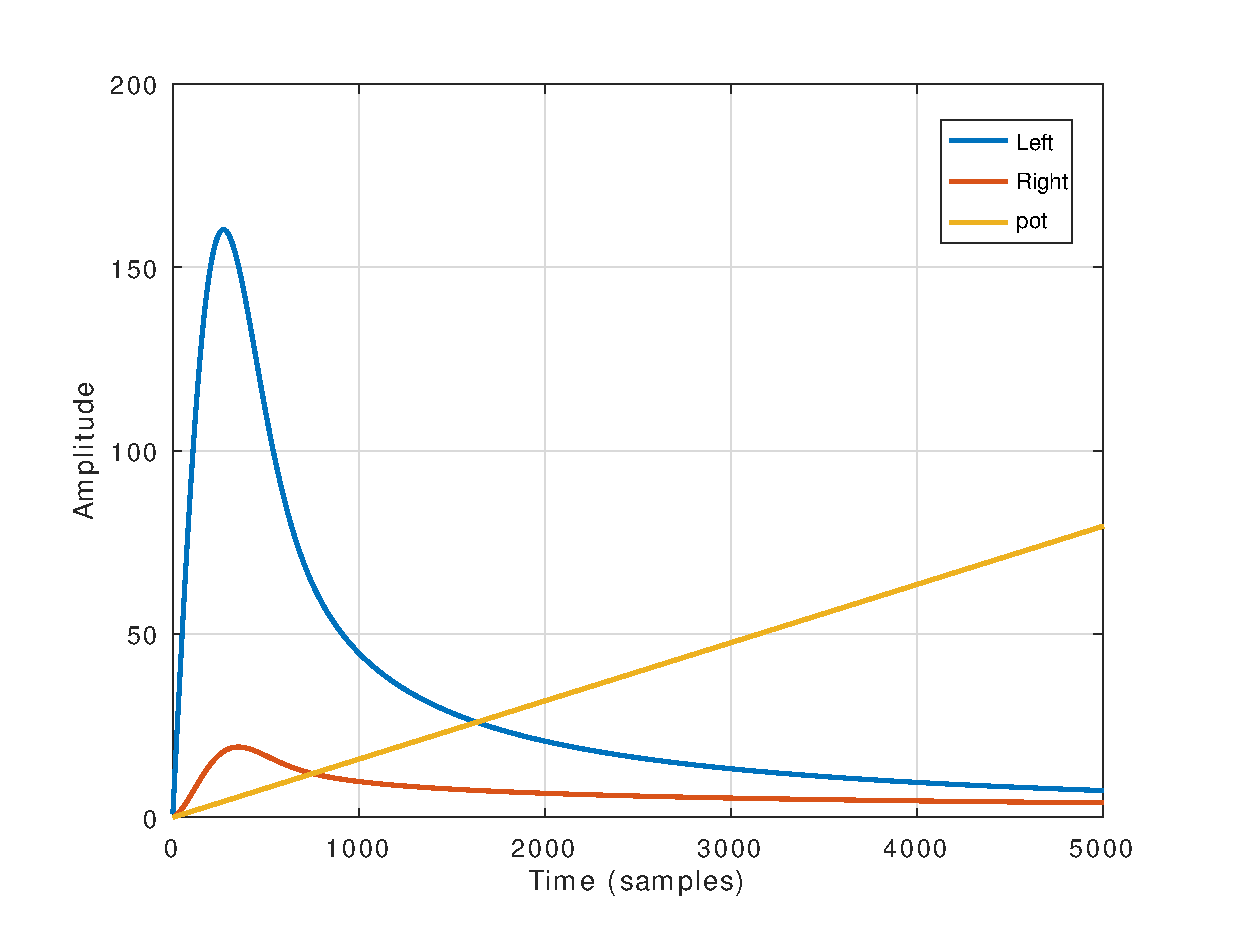
\includegraphics[width=1\columnwidth]{lrpanfb_init}
% % \caption{\textbf{Left-Right quadratic amplitude panner feedback response}. The plot shows panner response at one cycle of sweep from left to right. The plot shows as amplitude moves fast over 150 times the initial value on the “in-feedback” channel and over 20 times on the “opposite” channel.}
% % \label{fig:lrpanfb1}
% % \end{figure}
% %
% % \begin{figure}[t]
% % \centering
% % \includegraphics[width=1\columnwidth]{lrpanfbpot2}
% % \caption{\textbf{Left-Right quadratic amplitude panner feedback response}. The plot shows the moment in which the cycle of sweep pass from right through left and again reversing to right. It shows as amplitude moves fast over 300 times the initial value on the “in-feedback” channel and over 30 times on the “opposite” channel.}
% % \label{fig:lrpanfb2}
% % \end{figure}
% %
% % We have explained the path to Mid-Side panning, starting from the roots. Now it is the moment to understand what are the possible usages and what are the peculiarities of a Mid-Side panner instead of the \emph{traditional} amplitude panners.
% %
% % The \emph{matrixed} signal has its complexity as a disadvantage. Stop. In fact it requires knowledge and fantasy to understand a signal as the significance of matrix combination and it also requires a bit of tricky work more than a straight-signal.
% %
% % As musicians, even when plots and formulas appear pretty clear, in the end, at the moment of judgment, are the ears and the musical usability to determine the best, personal, choice.
% %
% % The fascinating realm of \emph{matrixed} signals forces a little to work by thought. So, for us, for example, the phase modulation strength of the Mid-Side panner had suggested, even before a practical test, better stability on live usages. Why? It is pretty simple to demonstrate.
% %
% % A microphone is routed into a channel, with a mid-lateral pointed panner, suppose 23 degrees to left and fed to the loudspeakers. With the quadratic panner, both left and right channels have different amplitude values with the same phase values. The feedback of the loudspeakers' signals inside the microphone comes from in-phase different energies sources. Searching the feedback with fingers on the gain will produce signals that will increase at least quadratically [fig. \ref{fig:lrpanfb1}, \ref{fig:lrpanfb2}].
% %
% % \begin{figure}[h]
% % \centering
% % 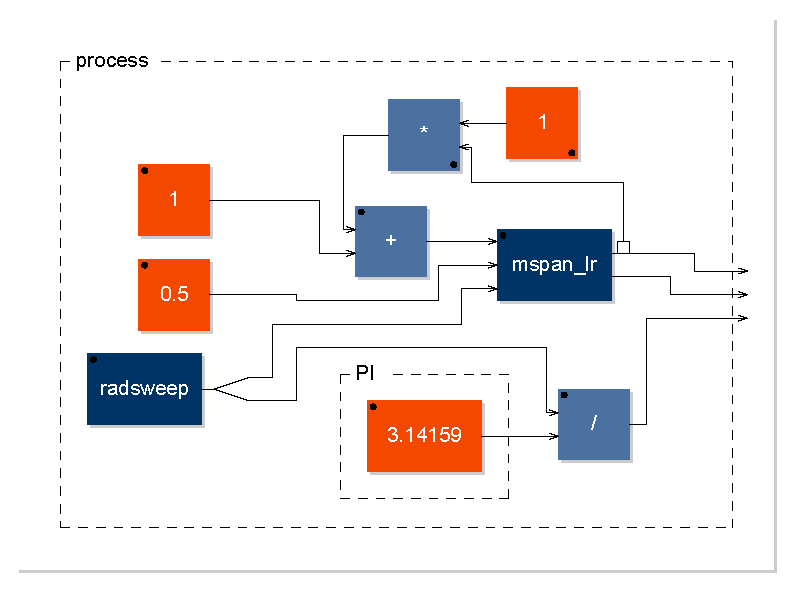
\includegraphics[width=1\columnwidth]{mspanlrfb_diagram}
% % \caption{\textbf{Block diagram of the infinite feedback}.}
% % \label{fig:mspan}
% % \end{figure}
% %
% % On the other hand, in the same feedback situation, with the same angular panning provenience applied to the microphone signal, the Mid-Side panning will produce different phase and different energy for both loudspeakers. The differences, in air, will produce a more resistive feedback pattern. In other words, the Mid-Side panner act "naturally" as anti-\emph{Larsen}.
% %
% % %\vfill\null
% % %\newpage
% %
% % %%%%%%%%%%%%%%%%%%%%%%%%%%%%%%%%%%%%%%%%%%%%%%%%%%%%%%%%%%%%%%%%%% SECTION SEVEN
% % %%%%%%%%%%%%%%%%%%%%%%%%%%%%%%%%%%%%%%%%%%%%%%%%%%%%%%%%%%%%%%%%%%%%%%%%%%%%%%%%
% % \section{CONCLUSIONS}
% % \label{sec:conc}
% %
% % \begin{figure}[t]
% % \centering
% % \includegraphics[width=1\columnwidth]{mspanlrfbpot}
% % \caption{\textbf{Mid-Side to Left-Right panner}. The plot describes the feedback response with a pan movement through the entire panorama, from -180 to 180 degrees (yellow line, normalized to -1 and 1). The energy multiplies up to four times for the left channel in infinite feedback (blue line). The top of feedback increasing is at 45 degrees position in direction of the channel in feedback.}
% % \label{fig:mspanlrfb}
% % \end{figure}
% %
% % This is the second article \emph{SEAM} produces to spread the music sustainability concept \cite{bevi05} from live electronics music to the broader electroacoustic music composition and interpretation. The original issues about music score documentation in electronic music are the fundamental core of the concept. Nevertheless, the focus of this research, and the approach, point to a compositional and practical situation that afflicts not only the documentation of a score but the musical thinking and practice at all.
% %
% % The research defines a critical educational situation, the first one analysed pretend to overcome literature with a new fancy way of teaching, writing books, in our opinion ludic, to educate like playing. There are a lot of textbooks, didactically introduced at each level of electronic music school, with the “doing, does not matter why" approach. You can pretty simply recognize them, they offer electronic music teaching as a collection of recipes, articulated like a foreign language book. Some authors praise themselves for the didactic unit-based structure of their books, inspired by foreign language learning texts. Is that music? Is music a foreign language? From these gruesome attitudes, the \emph{SEAM PROJECT} wants to take long-distance. What distance? Distance in thinking music and thinking about music, because sustainability is only superficially a technical issue. The documentation is a quality parameter of sustainability but it is the musical practicing and interpreting that will build musical thinking during the years.
% %
% % The first concept to be clarified in the conclusions is that sustainability must aim at maintaining a musical idea, the peculiarities of a concept is necessary like the peculiarities of the piece of art. We point at sustaining the speculation that music produces, through the sustaining of listening, that we have defined as the \emph{sustainability of the process}.
% %
% % %The paper also has a journey profile, conceived around the idea of speaking diagonally to different levels of electroacoustic learning.  The repertoire, the literature, needs people sharing their knowledge, to refine common conscience. A community can operate as a Research Group, with a “common appreciation of interdisciplinary problems” \cite{ml91}, to bring a time-frozen composition back to a warm and discussed work, out of a solipsistic production-in-a-box typical of the personal computing era, to focus on musical matters carved out on the personal knowledge, outside the personal point of view.
% %
% % It is necessary to focus on the main difference between technical sustainability and musical sustainability. Technical sustainability concerns the work, it is linked to the technical world that the work defines. It is its carbon dating, the reproducible ecosystem, maybe, but it is not the work itself. Musical sustainability is a matter of thoughts, that makes use of those tools to go out towards the perceptible. Supporting the thoughts is supporting music, perception, and listening.
% %
% % \begin{quote}
% % La musica non è solo composizione. Non è artigianato, non è un mestiere. La musica è pensiero \cite{nono85}\footnote{Music is not only about composing. It’s not handcraft, neither only a craft. Music is thought.}.
% % \end{quote}



%\appendix

%\chapter{PROGRAMMAZIONE V}

%\clearpage

%\begin{longtable}{r|L{0.71\textwidth}}
  \multicolumn{2}{c}{\textbf{CLASSE V LICEO MUSICALE • I Quadrimestre}} \\
  \multicolumn{2}{c}{\textbf{I modulo Titolo: Linguaggi di programmazione, interattività e multimedialità}} \\
  \endhead
  \hline
  \textbf{Obiettivi} &
  \textbf{Conoscenze:} \newline
    Acquisire i principali strumenti critici per l'analisi dell'audiovisivo.\newline
    Conoscere le principali tecniche di produzione e post-produzione audio e musicale in relazione all'audiovisivo.\newline
    Completare la conoscenza del percorso storico della musica elettroacustica, le aree territoriali, i compositori e le relazioni storiche tra essi.\newline
    Principi di interattività, installazione, realtà virtuale, multimedialità. \newline
  \textbf{Abilità:} \newline
    Lettura e comprensione di testi della letteratura specifica, manuali operativi e utente, di strumenti di lavoro, hardware e software.\newline
    Elaborazione e produzione di progetti compositivi, sia in forma di esercizio che di produzione autonoma, in lavori di gruppo con sistemi di condivisione dati e networking.\newline
    Accesso alla stesura di strutture musicali per gli audiovisivi e le opere interattive.\newline
    Elaborazione e produzione di un repertorio elettroacustico.\newline
  \textbf{Competenze:} \newline
    Completa padronanza della terminologia specifica, degli strumenti di studio, esercizio e lavoro applicato alle tecnologie musicali.\newline
    Completa autonomia critica ed analitica di opere elettracustiche e digitali.\newline
    Completa autonomia di produzione ed elaborazione personale spontanea e su commissione. \\
  \hline
  \textbf{Contenuti} &
    La tecnologia come strumento di esercizio e lavoro applicato alle
    discipline di studio. L'approfondimento teorico e la prova sperimentale
    come approccio d'indagine. Il repertorio musicale e la letteratura come
    guida tra le tematiche d'approfondimento. \newline
    Il computer come strumento e ambiente di lavoro polifunzionale.
    Il linguaggio di programmazione come strumento di pensiero. \newline
    L'elaborazione dei suoni al computer, elaborazione strutturata di un segnale,
    le tecniche di \emph{digital signal processing - dsp}.\newline
    La notazione musicale contemporanea, suono segno ed interpretazione.\newline
    Le superfici di controllo, le automazioni i sensori, strutturazione e
    programmazione di un proprio ambiente di lavoro personalizzato. \\
  \hline
  \textbf{Metodo} &
    Lezione frontale in laboratorio. \newline
    Ogni tematica è affrontata accedendovi dal repertorio musicale.
    Si ascolta, analizza e comprende il brano di repertorio ed attraverso
    la sua applicazione musicale si approfondiscono gli argomenti emergenti.
    Si veicola quindi lo studio teorico e tecnico attraverso la pratica
    musicale, senza perdere il collegamento con il repertorio storico.
    Ogni fenomeno uditivo, percettivo e tecnologico è radicato nella
    musica del suo tempo, acquisibile mediante l'analisi, l'interpretazione
    e la pratica dello strumento tecnologico musicale. \\
  \hline
  \textbf{Tempi} &
    Mesi da Settembre a Gennaio\\
  \hline
  \textbf{Materiali} &
    Dispense, Estratti di testi in letteratura, partiture del repertorio,
    contenuti multimediali. \\
  \hline
  \textbf{Tipologia della verifica} &
    Prove pratiche sulle attività svolte durante i laboratori. \newline
    Questionari di diversa tipologia. \newline
    Verifiche orali.
\end{longtable}%

\clearpage

\begin{longtable}{r|L{0.71\textwidth}}
  \multicolumn{2}{c}{\textbf{CLASSE V LICEO MUSICALE • II Quadrimestre}} \\
  \multicolumn{2}{c}{\textbf{II modulo Titolo: Musicista e Tecnologia, competenze trasversali.}} \\
  \endhead
  \hline
  \textbf{Obiettivi} &
    \textbf{Conoscenze:} \newline
      Acquisire i principali strumenti critici per l'analisi dell'audiovisivo.  \newline
      Conoscere le principali tecniche di produzione e post-produzione audio e musicale in relazione all'audiovisivo.  \newline
      Completare la conoscenza del percorso storico della musica elettroacustica, le aree territoriali, i compositori e le relazioni storiche tra essi.  \newline
      Conoscenza delle pratiche di interattività, installazione, realtà virtuale, multimedialità.  \newline
    \textbf{Abilità:} \newline
      Elaborazione e produzione di progetti compositivi, relazioni, articoli scientifici e documentazione operativa, partiture e schede tecniche. \newline
      Elaborazione e produzione di strutture musicali per gli audiovisivi e le opere interattive.\newline
      Elaborazione e produzione di un repertorio elettroacustico. \newline
    \textbf{Competenze:} \newline
      Completa padronanza della terminologia specifica, degli strumenti di studio, esercizio e lavoro applicato alle tecnologie musicali. \newline
      Completa autonomia critica ed analitica di opere elettracustiche e digitali. \newline
      Completa autonomia di produzione ed elaborazione personale spontanea e su commissione. \\
    \hline
    \textbf{Contenuti} &
      La tecnologia come strumento di esercizio e lavoro applicato alle
      discipline di studio. L'approfondimento teorico e la prova sperimentale
      come approccio d'indagine. Il repertorio musicale e la letteratura come
      guida tra le tematiche d'approfondimento. \newline
      Il computer come strumento e ambiente di lavoro polifunzionale. \newline
      Il linguaggio di programmazione come strumento di pensiero. \newline
      L'elaborazione dei suoni al computer, elaborazione strutturata di un segnale,
      le tecniche di \emph{digital signal processing - dsp}. \newline
      La notazione musicale contemporanea, suono segno ed interpretazione. \newline
      Studio, ricerca e produzione, acquisizione dei mezzi per sviluppare il
      proprio percorso musicale. \\
    \hline
    \textbf{Metodo} &
      Lezione frontale in laboratorio. \newline
      Ogni tematica è affrontata accedendovi dal repertorio musicale.
      Si ascolta, analizza e comprende il brano di repertorio ed attraverso
      la sua applicazione musicale si approfondiscono gli argomenti emergenti.
      Si veicola quindi lo studio teorico e tecnico attraverso la pratica
      musicale, senza perdere il collegamento con il repertorio storico.
      Ogni fenomeno uditivo, percettivo e tecnologico è radicato nella
      musica del suo tempo, acquisibile mediante l'analisi, l'interpretazione
      e la pratica dello strumento tecnologico musicale. \\
    \hline
    \textbf{Tempi} &
      Mesi da Febbraio a Giugno \\
    \hline
    \textbf{Materiali} &
      Dispense, Estratti di testi in letteratura, partiture del repertorio,
      contenuti multimediali. \\
    \hline
    \textbf{Tipologia della verifica} &
      Prove pratiche sulle attività svolte durante i laboratori. \newline
      Questionari di diversa tipologia. \newline
      Verifiche orali. \newline
      Presentazione della produzione personale acquisita durante l'anno scolastico. \newline
      Prova pratica interpretazione d'insieme in forma di concerto.
  \end{longtable}%

\clearpage

\begin{longtable}{R{0.21\textwidth}|L{0.71\textwidth}}
\multicolumn{2}{c}{\textbf{CRITERIO DI SUFFICIENZA}} \\
\endhead
\hline
\multicolumn{2}{c}{L’alunno conseguirà la valutazione sufficiente quando dimostrerà di possedere:} \\
\hline
\multicolumn{2}{c}{\textbf{Nel I Quadrimestre:}} \\
\hline
Conoscenze: &
Conoscenza completa delle discipline in oggetto, del lessico specifico, degli strumenti di lavoro. \\
\hline
Abilità: &
Capacità di gestione autonoma di attività tecniche e pratiche all'interno del laboratorio, individuali e collettive. \\
\hline
Competenze: &
Competenza e lessico appropriato nel rapporto con gli strumenti di lavoro e le tecnologie. \newline
Competenza dell'ambiente virtuale al computer, dell'acquisizione e trattamento digitale dei suoni. \newline
Autonomia critica, analitica e di giudizio, d'ascolto e relazione con la musica e i media. \\
\hline
\multicolumn{2}{c}{\textbf{Nel II Quadrimestre:}} \\
\hline
Conoscenze: &
Conoscenza completa delle discipline in oggetto, del lessico specifico, degli strumenti di lavoro. \\
\hline
Abilità: &
Capacità di gestione autonoma di attività tecniche e pratiche all'interno del laboratorio, individuali e collettive. \\
\hline
Competenze: &
Competenza e lessico appropriato nel rapporto con gli strumenti di lavoro e le tecnologie. \newline
Competenza dell'ambiente virtuale al computer, dell'acquisizione e trattamento digitale dei suoni. \newline
Autonomia critica, analitica e di giudizio, d'ascolto e relazione con la musica e i media.
\end{longtable}

\clearpage


\clearpage

\printbibliography

\clearpage

\listoffigures

\clearpage

\listoftables

\clearpage

%\listofformulas

\addcontentsline{toc}{chapter}{Indice dei nomi}
\printindex

\end{document}
